%You can delete all the comments after you have finished your document
%this sets up the defaults for the documents, 12pt font and A4 size. The article type sets this up as such as opposed to letter or memo.

%for the finer points LaTeX see https://en.wikibooks.org/wiki/LaTeX or http://tex.stackexchange.com/

\documentclass[12pt,a4paper]{article}
\usepackage{titlesec} %these are how we import packages, one helps set up footers and title layout
\usepackage{fancyhdr}

% !TEX TS-program = pdflatex
% !TEX encoding = UTF-8 Unicode
\usepackage[utf8]{inputenc} % set input encoding (not needed with XeLaTeX)

\usepackage{graphicx} % support the \includegraphics command and options
\graphicspath{ {images/} } % tells LATEX that the images are kept in a folder named images under the current directory.

% \usepackage[parfill]{parskip} % Activate to begin paragraphs with an empty line rather than an indent

%%% PACKAGES
\usepackage{booktabs} % for much better looking tables
\usepackage{array} % for better arrays (eg matrices) in maths
\usepackage{paralist} % very flexible & customisable lists (eg. enumerate/itemize, etc.)
\usepackage{verbatim} % adds environment for commenting out blocks of text & for better verbatim
\usepackage{subfig} % make it possible to include more than one captioned figure/table in a single float
\usepackage[toc,page]{appendix}
% These packages are all incorporated in the memoir class to one degree or another...
\usepackage{pdfpages}
% Testing to see how IPO will look as I use this and use it as a pdf
\usepackage{csquotes}
%" facing the wrong way so trying to rectify that

\usepackage[breaklinks = true]{hyperref}
\hypersetup
{
	colorlinks=false, %set true if you want colored links
	linktoc=all,     %set to all if you want both sections and subsections linked
}
%\usepackage[hyphenbreaks]{breakurl}
\usepackage[anythingbreaks]{breakurl}
\usepackage{gensymb}
\usepackage[round]{natbib}

\usepackage{tabu}

%header and footer settings
\pagestyle{fancyplain}
\fancyhf{}
\renewcommand{\headrulewidth}{0.5pt}
\renewcommand{\footrulewidth}{0.5pt}
\setlength{\headheight}{15pt}
\fancyhead[L]{Ryan O'Flaherty - 40168766}
\fancyhead[R]{SOC10101 Honours Project}
\fancyfoot[L]{}
\fancyfoot[C]{\thepage}

%set better section layout
\makeatletter
\renewcommand\subsection{\@startsection {subsection}{1}{2mm} % name, level, indent
                               {3pt plus 2pt minus 1pt} % before skip
                               {3pt plus 0pt} % after skip
                               {\normalfont\bfseries}}
\makeatother
\makeatletter
\renewcommand\section{\@startsection {section}{1}{0mm} % name, level, indent
                               {4pt plus 2pt minus 1pt} % before skip
                               {4pt plus 0pt} % after skip
                               {\bfseries}}
\makeatother


%this starts the document
\begin{document}

%you can import other documents into your main one, these layout the Title and Declarations on its own page.
%you might need to change these to \ if your on Microsoft Windows.
\newcommand{\HRule}{\rule{\linewidth}{0.5mm}}

\begin{titlepage}
	\begin{center}

	\HRule \\[0.4cm]
    	{\Large \bfseries Evolution of Neural Network Controllers\\for Gameplay Behaviours\par}
	\vspace{0.2cm}
	\HRule \\[1.5cm] 

	
    	\vspace{3cm}
	\begin{minipage}{0.4\textwidth}
	\begin{center} \large
        \emph{}\\
        	Ryan O'Flaherty 40168766
				
   	 \end{center}
    	\end{minipage}
	
	\vspace{2cm}
    	\begin{minipage}{1\textwidth}
    	\begin{center} \large
        
		Submitted in partial fulfilment of \\
		the requirements of Edinburgh Napier University \\
		for the Degree of \\
        	BSc (Hons) Games Development
    	\end{center}
    	\end{minipage}

    	\vfill

    	% Bottom of the page
	\begin{minipage}{1\textwidth}
    	\begin{center} \large
		School of Computing
    	\end{center}
    	\end{minipage}
	
	\vspace{1cm}
    	{\large \today}


	\end{center}
\end{titlepage}
%{\large Submitted in partial fulfilment of the requirements of Edinburgh Napier University for the Degree of }
\clearpage
\section*{Authorship Declaration}
\vspace{0.5cm}
\begin{flushleft}
I, Ryan O'Flaherty, confirm that this dissertation and the work presented in it are my own achievement.\newline

Where I have consulted the published work of others this is always clearly attributed;\newline

Where I have quoted from the work of others the source is always given. With the exception of such quotations this dissertation is entirely my own work;\newline

I have acknowledged all main sources of help; \newline

If my research follows on from previous work or is part of a larger collaborative research project I have made clear exactly what was done by others and what I have contributed myself;\newline

I have read and understand the penalties associated with Academic Misconduct.\newline

I also confirm that I have obtained informed consent from all people I have involved in the work in this dissertation following the School's ethical guidelines.\newline
\end{flushleft}

\begin{flushleft} \large
\emph{Signed:} \\
\end{flushleft}

\vspace{.5cm}

\begin{flushleft} \large
\emph{Date:} \\
\end{flushleft}

\vspace{.5cm}

\begin{flushleft} \large
\emph{Matriculation no: }  \\
\end{flushleft}
\thispagestyle{empty}
\pagebreak
\clearpage
\section*{Data Protection Declaration}
\vspace{0.5cm}
\begin{flushleft}
Under the 1998 Data Protection Act, The University cannot disclose your grade to an unauthorised person. However, other students benefit from studying dissertations that have their grades attached. \newline

\vspace{0.5cm}

Please sign your name below one of the options below to state your preference.\newline
\vspace{0.5cm}

The University may make this dissertation, with indicative grade, available to others.\newline
\vspace{3cm}


The University may make this dissertation available to others, but the grade may not be disclosed.\newline
\vspace{3cm}


The University may not make this dissertation available to others.\newline
\end{flushleft}


\thispagestyle{empty}
\pagebreak

\pagenumbering{roman}
\setcounter{page}{1}

%LaTeX let you define the abstract separately so it wont get sucked into the main document.
\begin{abstract}
\
% fill the abstract in here
$\\ \clubsuit \\\\ \diamondsuit \\\\ \heartsuit \\\\ \spadesuit$

Original NEAT publication:\\
http://nn.cs.utexas.edu/downloads/papers/stanley.ec02.pdf\\\\

Couldn't find the tutorial but I stuck it on my website:\\
http://x4iiiis.com/honours/NEATDOC.pdf

Actually it's in the download here, as a .ps 
http://nn.cs.utexas.edu/soft-view.php?SoftID=4



\end{abstract}
\pagebreak

%\pagenumbering{arabic}
%\tableofcontents % is generated for you
%\pagenumbering{roman}
\newpage



\cleardoublepage
% Let's change \thepage so it prints one less than
% the real page number; \pagenumbering{arabic}
% will redefine it to the right meaning afterwards.
\renewcommand\thepage{\romannumeral\numexpr\value{page}\relax}

\tableofcontents

\cleardoublepage

\listoftables
%generated in same way as figures
\newpage

\listoffigures
%you may have captions such as equations, listings etc they should all appear as required
%these are done for you as long as you use \begin{figure}[placement settings] .. bla bla ... \end{figure}
\newpage

\section*{Acknowledgements}
%The Games Development course has been journey of personal development in addition to gaining a higher education by obtaining and improving skills. It has been the proverbial roller-coaster ride with several highs, lows, moments of complete disorientation, and a feeling of wishing you could do it all over again. The last four years have gone by in the blink of an eye, but have provided experiences and created friendships that will remain far beyond graduation.\\


%I would like to thank my friends and family for ensuring that I remained positive and motivated along the way, and for their participation in the testing phases. All of the support, assistance and feedback has been invaluable to both myself and the project as a whole. \\

%I am also hugely appreciative of my project supervisor, Dr Simon Powers. Simon has provided me with excellent support and guidance throughout the process and for that I am extremely grateful.

I would like to thank Calum and Steven for abstaining from Fortnite duties on the night of 24/03/18 as not having my squaddies meant actually fixing this fucking thing.

Also, cheers to my supervisor, I suppose. 

\newpage
\setcounter{page}{1}
\pagenumbering{arabic}

\section{Introduction}

% Jyoti's advice
Jyoti's advice\\\\
% 1 
background to topic
rationale for project
x2 paragraphs\\

\subsection{1.2 - Aims and Objectives}
Aim and objectives
Aim is one sentence (the deliverable)
In order to reach this goal, the following objectives will be achieved:
- etc
- etc

\subsection{1.3 - Scope}
Scope
Don’t let them ask you at the viva voce “why didn’t you build it for X” 

\subsection{1.4 - Constraints}
Constraints
Everyone has time constraints so don’t be a dickhead

\subsection{1.5 - Sources of Information (~/Similar Work)} 
Sources of information ( ~/similar work )
C++ (11) 
NEAT
SMFL\\\\

Sixteen years prior to this project, researchers(?) at The University of Texas at Austin published a paper in which they detailed the development of their innovative neural network evolution library\citep{NEAT} entitled, \enquote{NeuroEvolution of Augmenting Topologies,} or \enquote{NEAT} in abbreviated form. The library has been converted to several programming languages over the years; However this project will stick with the original C++ version. The NEAT library will be discussed in depth in the Methodology section of this dissertation.\\

This project will be built in C++, and will need to be compiled to a minimum of C++11 standard due to the use of shared pointers.\\

Visual aspects of the project will be developed with SFML imported.\\

\subsection{1.6 - Chapter Outlines / Structure of Dissertation}
Chapter outlines / structure of dissertation
Chapter 1 contains intro
Chapter 2 contains
Chapter 3 … \\

% end of Jyoti's advice
end of Jyoti's advice\\\\

This chapter highlights the aims and objectives for this honours project, providing a brief insight into the what is to come. It also outlines the desired deliverables for the completed project. \\

\subsection{Project Aims and Structure}
%Or have sections that are relevant to your main body of work above but warrant their own section. Both - with numbering would be entered into the Table of contents.

This project intends to provide a digitally playable card game that can be played by a human user against one or more artificial intelligence agents. The underlying purpose of the project is to research and demonstrate the effectiveness of artificial neural networks and evolutionary algorithms in a game of this type. 

It plans to do so by using the NeuroEvolution of Augmenting Topologies (NEAT) library to co-evolve neural network structures as well as input weights to make decisions relating to in-game moves that can be made, and to learn from the results of those decisions. 

This report will document how well the agent performs over a vast amount of games and topologies, presenting the results through a mixture of figures and charts. An in-depth explanation of the way in which the performance is measured will be described in the methodology section. 

While the project has research at its core, it is also intended to be a game that can provide an enjoyable experience for a playing user who may not appreciate what is going on under the hood.\\

 \subsection{Overview Of Project Content and Milestones}

Milestone proposals for the project are as follows: 
\subsubsection{Research}
Neural networks and Evolutionary algorithms research is necessary to aid with the project development and to make up for current lack of knowledge

\subsubsection{Game Foundation}
A short-term goal of the project is to create a bare-bones version of the card game without any artificial intelligence. This has to be created as it is the foundation on which the rest of the project will reside, and as such it needs to be rigorously tested to ensure that the rules of the game have been correctly implemented without any bugs. That way, any future problems will be related to the artificial intelligence itself.

\subsubsection{Implementation of Artificial Intelligence}
Most likely the phase of greatest difficulty and complexity, the implementation of artificial neural networks and evolutionary algorithms is expected to be a largely time consuming task. 

This will be where the game will transition from a hard-coded, bare-bones implementation to something of more interest. Once this has been successfully set up, we can begin testing and tweaking it to analyse the varying results.

\subsubsection{Experiments and Testing}
A large amount of games will be required to allow the evolution process to grow into something that performs to a decent level in our game. This will mean the game will have to be played multiple times, and so it will be beneficial to get other people to play-test the game too. 

Each time tweaks are made in our algorithm, the game will need to be thoroughly re-tested, with the results of these tests being accurately documented to provide a solid basis for the next stage of tweaking. 

The aim is to have a very large set of data to analyse and draw conclusions from in the latter stages of the project. 

\subsubsection{Evalution and Conclusion}
The aforementioned dataset will be used extensively to deeply examine the performance of each machine learning techniques implemented throughout the experimental stage of the project, with regards to both our hard-coded solutions and the results of other attempted solutions. 

\newpage
\section{Background}
\subsection{Introduction}
The following section of this dissertation will go on to discuss the history of artificial intelligence within the context of video games, before going on to explain neural networks, evolutionary algorithms, and the NeuroEvolution of Augmenting Topologies (NEAT) library.\\

\subsection{History of AI in Games}
Video games have been a popular area of interest for artificial intelligence developers and researchers for many decades. 

Over several tens of years, a large amount of research and development has been done in an attempt to perfect chess-playing artificial intelligence agents\citep{L2PChess}, and work has more recently been put in to do the same with the game of Go.  

In March of 2016, the goal of getting such an agent to compete and win at the highest level was reached when AlphaGo, a program engineered by Google, managed to overcome the Go world champion human player, Lee Sedol\citep{ABriefHistoryOfGameAI}. This was then reported as a major breakthrough for the artificial intelligence field. 

With Go, developers are unable to use brute force approaches due to the vastly complex nature of the game\citep{13}. In other words, the complexity of Go means that a strategy cannot be hard-coded to play the game, and things like search trees are not applicable either. AlphaGo's solution to this was the implementation of a neural network to learn and play the game, taking into consideration millions of game states from previous games involving human expert players. 

This would theoretically result in AlphaGo performing at a similar level to that of the human players it learned from. To go above and beyond that level, and to be able to beat a champion like Sedol, AlphaGo was then put up against itself, consequently improving with every game it played\citep{13}. It can be said that in this phase, AlphaGo literally taught itself. 

In terms of Chess, a machine managed to win against a human of World Champion status named Gerry Kasparov in the late 1990s\citep{14}. That machine was Deep Blue. In actual fact, it was the second version of IBM's Deep Blue. The first Deep Blue lost to the same opponent a year prior to it's successor's achievement in 1997\citep{14}. That success came in the form of two wins, a loss, and three draws\citep{15}, over the course of several days. However, IBM did not use artificial intelligence with Deep Blue, relying instead on computational power and a less complex search and evaluation function\citep{16}. \\

\subsection{What is a Neural Network?}
Artificial neural networks, commonly referred to simply as neural networks, are a rough representation of the human brain. Human brains can be thought of as highly complex and non-linear systems for processing information in parallel\citep{NeuralNetworksAComprehensiveFoundation}. 

To emulate this, neural networks are built using a series of layers of network nodes. These nodes are used to represent neurons in the brain. The first is an input layer, followed by two or three hidden layers before a final output layer of nodes\citep{ArtificialNeuralNetwork}. The connection between these nodes is representative of axons in the brain. 

In an artificial neural network, the input and output layers take data in and produce results respectively, with the processing of said data being done within the hidden layers - but how does it work? 

\subsubsection{Perceptrons}
One type of artificial neuron (or node) is known as a \enquote{perceptron.} Each perceptron receives several inputs and uses them to produce one binary output\citep{NeuralNetworksAndDeepLearning}.  

\begin{figure}[h]
	\centering
	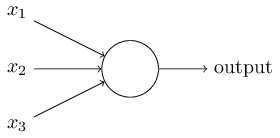
\includegraphics{Perceptron.png}
	\caption{A Single Perceptron}
\end{figure}

Frank Rosenblatt, the scientist who developed the perceptron in the 1950s and 1960s, devised a rule for computing the output from these neurons. Using what he called \enquote{weights,} the importance of each input is assessed and expressed. Each input has a weight assigned to it, and the resultant output from these inputs - either a 1 or 0 - is dependent on whether or not some threshold value is less than or greater than the sum of the weights from all of the inputs to that particular perceptron. Therefore, if the weighted sum is less than or equal to the threshold value, the output is a 0. Otherwise, a 1\citep{NeuralNetworksAndDeepLearning}. Both the threshold value and the input weights are real numbers. These can be tweaked to alter the decisions made by a neural network. 

\subsubsection{Sigmoid Neurons}

Sigmoid neurons are akin to perceptrons, however, they are modified in such a way that marginal alterations in their weights and bias cause only a small change to their output\citep{NeuralNetworksAndDeepLearning}. This crucial difference is what affords a network consisting of sigmoid neurons the ability to learn.

The inputs to a sigmoid neuron also differ from those of perceptrons. Rather than being binary (1 or 0), these inputs are any number \textit{between} 1 and 0. %probably pointless italics
Much like with perceptrons, these sigmoid neuron inputs are weighted, with an overall bias included. 

The shape of a plotted sigmoid function ($\sigma$) can be seen in Figure 2. 

\begin{figure}[h]
	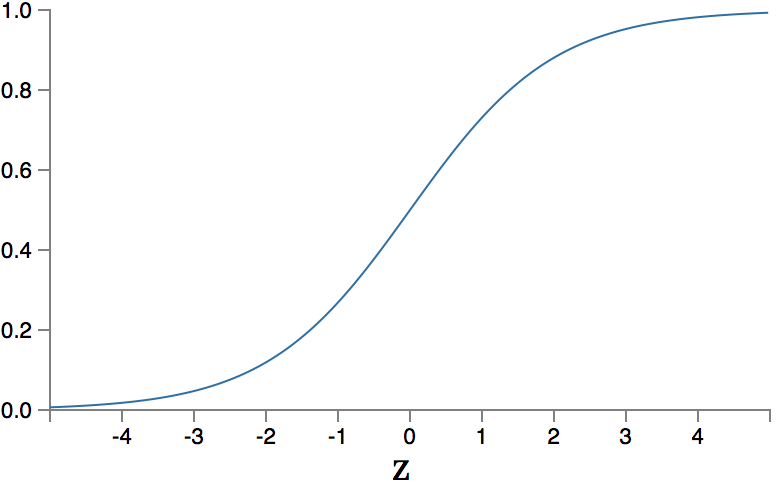
\includegraphics[width=\textwidth, height=5cm]{SigmoidFunction.png}
	\caption{Sigmoid Function} \centering{\citep{NeuralNetworksAndDeepLearning}}
\end{figure}

To give sigmoid neurons the smoothness required for a non-linear activation function, the following logistic function defining sigmoidal non-linearity is used:
\begin{eqnarray}
y_j = \frac{1}{1+exp(-v_j)}
\end{eqnarray}

\begin{center}
	\citep[Chapter 4, page 179] {NeuralNetworksAComprehensiveFoundation}
\end{center}

This calculates the output from our neuron \textit{{$y_j$}}, with \textit{j} being the neuron itself, and \textit{$v_j$} representing the sum of all inputs (with weighting applied) plus the bias\citep{NeuralNetworksAComprehensiveFoundation}.

Input weights can be calculated via the dot product. Thus, using \textit{w}, \textit{x} and \textit{b} as symbols for weights, inputs and bias, we can represent $v_j$ as 
\begin{eqnarray}
(w \cdot x+b).
\end{eqnarray}

\begin{center}
	\citep{NeuralNetworksAndDeepLearning}
\end{center}

Therefore, extending the output calculation gives us
\begin{eqnarray} 
%y_j = \frac{1}{1+\exp(-\sum_j w_j x_j-b)}.\\\\
y_j = \frac{1}{1+\exp(-\sum_j w_j \cdot x_j - b)}.
\end{eqnarray}


When $v_j$ is a large, positive number the sigmoid neuron output is approximately 1. On the other hand, the output is approximately 0 if $v_j$ is heavily negative. These outputs are similar to that of perceptrons. However, when $v_j$ is somewhere in between, the similarities cease. 

Even the smallest alterations to the weighting or bias can create small changes to the output from a sigmoid neuron, due to the smooth nature of the function\citep{NeuralNetworksAndDeepLearning}.\\

\subsection{Evolutionary Algorithms}
As the name might suggest, an evolutionary algorithm is one that evolves. It does so to encourage finding the most optimal solution to a problem. A vast amount of varying evolutionary algorithms exist, but at the core of them all is the same principal idea: \enquote{given a population of individuals the environmental pressure causes natural selection (survival of the fittest) and this causes a rise in the fitness of the population}\citep{IntroductionToEvolutionaryComputing}. As a result, the population adapts over time to its environment. 

What is the process of evolution? The generational cycle works as follows:

\subsubsection{Representation}
Step one when defining an evolutionary algorithm is to bridge the gap between the \enquote{real world} and the \enquote{evolutionary algorithm world}\citep{IntroductionToEvolutionaryComputing}. That is, to link what are known as phenotypes, to representative genotypes. 

%In order to use an evolutionary algorithm, possible solutions must be represented as what are known as chromosomes (or genotypes). 

\begin{itemize}
	\item Phenotype: A solution to a problem
	\item Genotype: Chromosome used to represent the solution to a problem
\end{itemize}

Representation refers to specifying which genotypes equate to each phenotype\citep{IntroductionToEvolutionaryComputing}. For example, if an integer is the solution to a problem, it is the phenotype, and a binary representation of that particular integer would be the genotype relating to that phenotype. 

A genotype (or chromosome) is made up of genes. Values are assigned to each gene, and may be referred to as alleles. These can be of any type, or even a mixture. Types include binary strings, integers, real values, permutations and symbols. So in the example above, each gene would be either a 1 or 0, combining to form the integer as an overall chromosome.

Sometimes it may not be quite so straightforward, and genotypes need to be explicitly mapped to phenotypes, as seen in Figure 3. 

\begin{figure}[h]
	\centering
	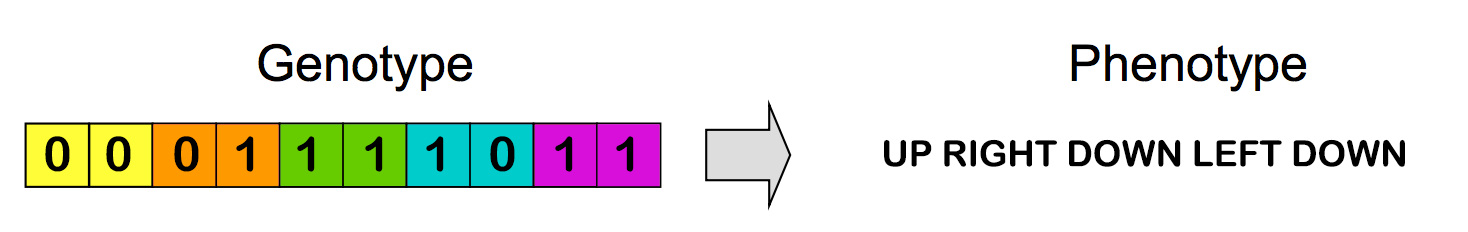
\includegraphics[width = \textwidth]{GenoToPheno.png}
	\caption{Genotype vs Phenotype}
\end{figure}


\subsubsection{Initialisation}
In the beginning, we start off with a population comprised completely of random chromosomes. This is likely to yield very poor results, however there is always a chance that some may be better. These individuals must then be evaluated.

\subsubsection{Fitness}
The fitness of an individual is what defines how fit for purpose it is. This measurement of quality will be defined differently for every algorithm, depending entirely on the context of problems it is being used to solve. In this project, the fitness will correlate to the amount of illegal moves the agent attempts to make, and how many times it is forced to increase its hand rather than decrease it. However, as the game of switch is largely down to luck, this will have to be taken into account to incorporate some form of leniency to fitness calculations.  

The role of an evaluation function (or fitness function) to encourage improvements by defining what an improvement is\citep{IntroductionToEvolutionaryComputing}. This lays the foundation for selection. 

\subsubsection{Selection}
The process of choosing individuals, based on their fitness, from the population to become parents to the next generation of individuals is called selection\citep{IntroductionToEvolutionaryComputing}. This is the driving force behind progressive evolution as it biases selection towards individuals of higher quality. 

\subsubsection{Crossover}
Sometimes referred to as recombination, crossover is an operation that merges genes from two parent genotypes together into one or two offspring genotypes\citep{IntroductionToEvolutionaryComputing}. 

Crossover can be defined in a few ways. There is one-point crossover, where a randomly chosen point along the length of a chromosome determines which genes are passed on from that particular genotype, and the rest will come from the other parent. This is demonstrated in Figure 4.

\begin{figure}[h]
	\centering
	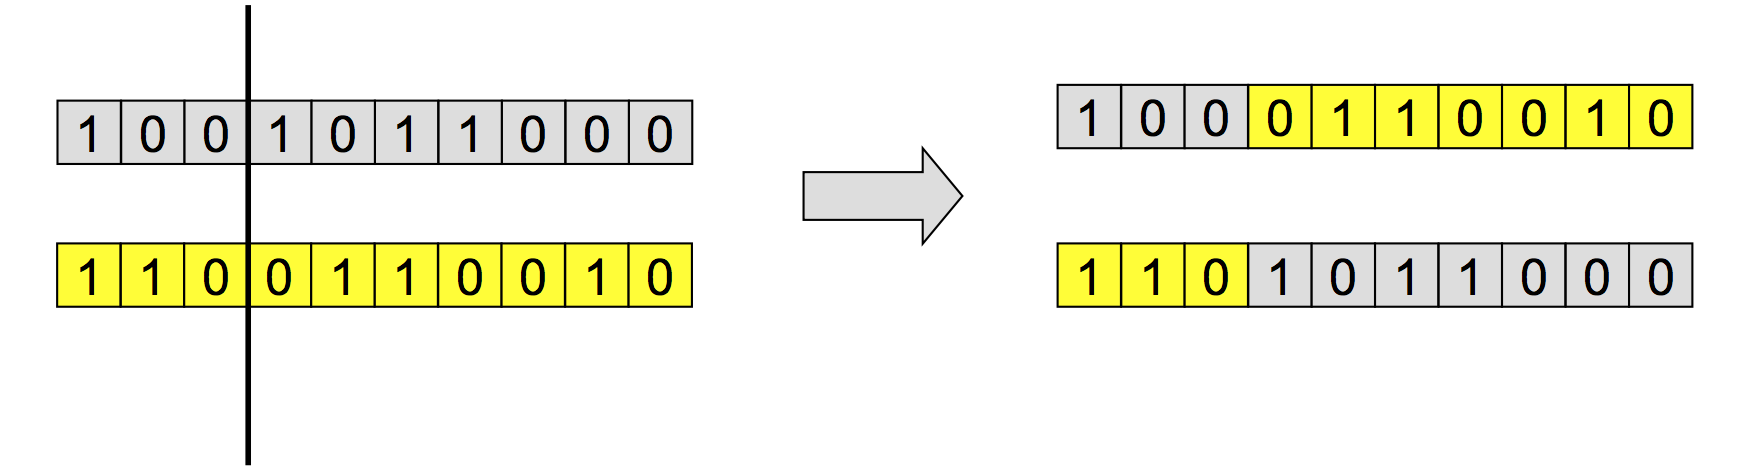
\includegraphics[width = \textwidth]{OnePointCrossover.png}
	\caption{One-Point Crossover}
\end{figure}

Next, n-point crossover is when more than one (n) point is chosen, and chromosomes can be split up in different ways, as seen in Figure 5. 

\begin{figure}[h]
	\centering
	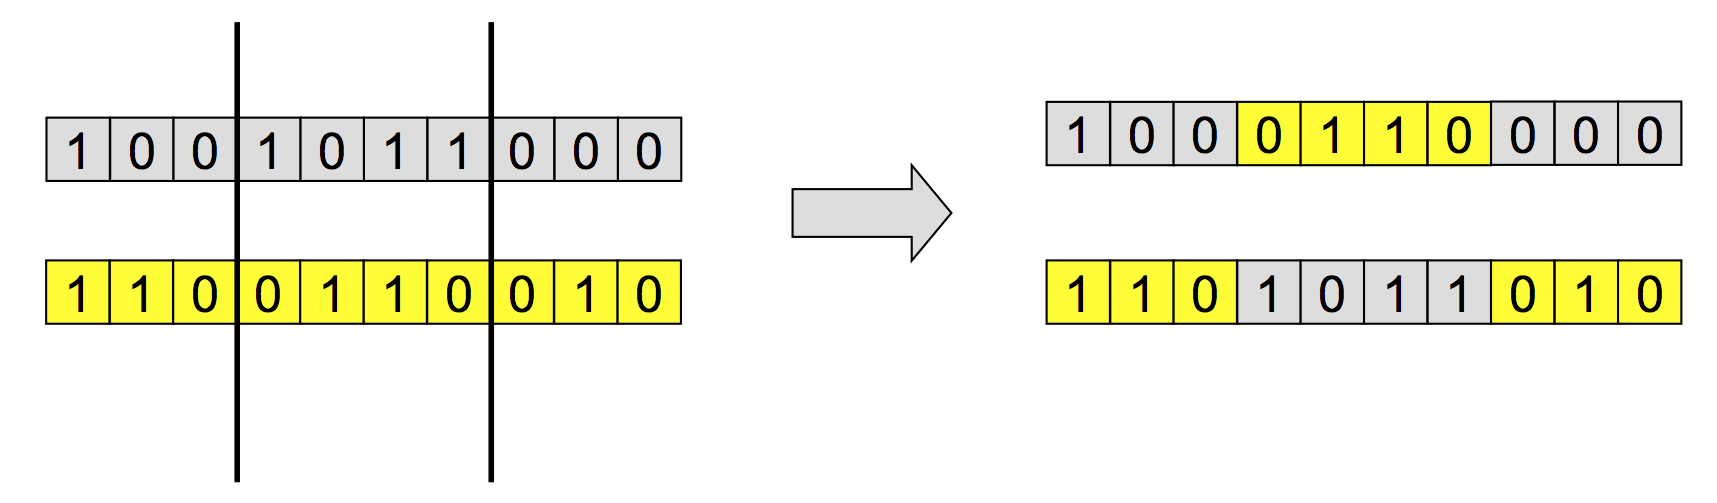
\includegraphics[width = \textwidth]{NPointCrossover.png}
	\caption{N-Point Crossover}
\end{figure}

Another type of crossover is called uniform. In this case, each gene of the offspring is randomly selected by deciding which of the two parents to inherit from. This is demonstrated in Figure 6.

\begin{figure}[h]
	\centering
	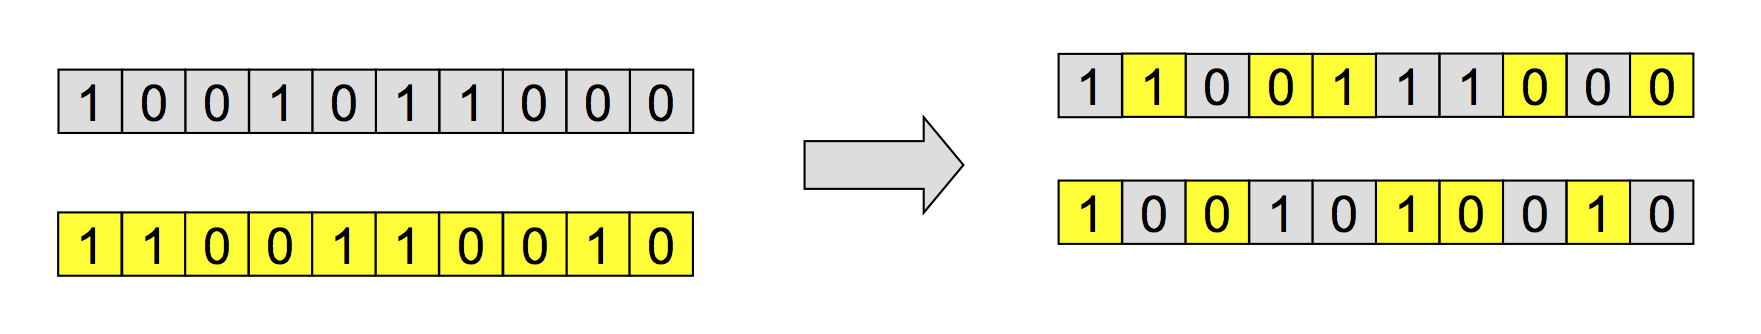
\includegraphics[width = \textwidth]{UniformCrossover.png}
	\caption{Uniform Crossover}
\end{figure}


In the case of arithmetic crossover, an average of the two parent genes is calculated and used for the child gene. This is useful if the genes consist of real numbers. Figure 7 depicts this.

\begin{figure}[h]
	\centering
	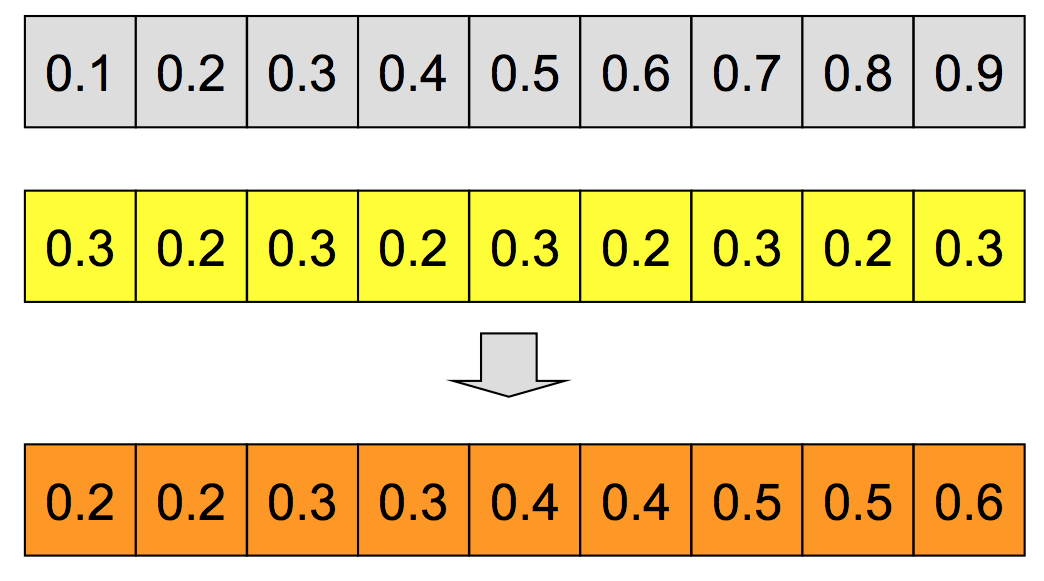
\includegraphics[width = \textwidth]{ArithmeticCrossover.png}
	\caption{Arithmetic Crossover}
\end{figure}

All of the above techniques are used in binary and integer chromosome representations. Permutations cannot be recombined using any of these techniques, but are beyond the scope of this project. 

\subsubsection{Mutation}
When applied to a genotype, mutation returns a slightly mutated offspring\citep{IntroductionToEvolutionaryComputing}. It can create new genes in the population, which in turn diversifies the population. 

Like with crossover, there are different ways to perform mutation. In the case of binary chromosomes, we would allow each gene to 'flip' from a 1 to a 0 or vice versa, as demonstrated by Figure 8. Each gene has a probability of being mutated in this way, which will often be calculated as 1/\textit{n} with \textit{n} being representative of the chromosome length.


%Binary
\begin{figure}[h]
	\centering
	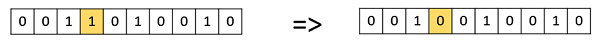
\includegraphics[width = \textwidth]{BinaryMutation.png}
	\caption{Binary Mutation}
\end{figure}

Integers are slightly different. The probability is remains the same, but the difference is that a set of possible numbers, for example 0 to 9, is set up and when a gene is chosen for mutation, a number within that range is randomly generated and used in the offspring. This is displayed in Figure 9.\\

%Integer
\begin{figure}[h]
	\centering
	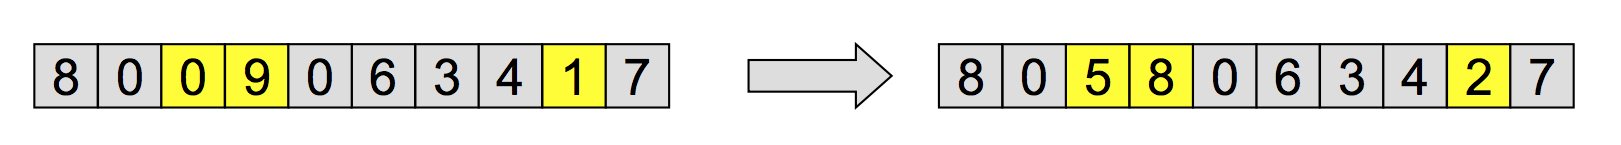
\includegraphics[width = \textwidth]{IntegerMutation.png}
	\caption{Integer Mutation}
\end{figure}
 
Again, permutations work in a completely different way, but are not considered as part of this project. 

\subsubsection{Replacement}
This is the part where individuals are removed from the population to make way for a generation of new and hopefully improved genotypes. We could just remove the oldest genotype in the population, but this could be one with a high fitness! This can also be done randomly, but again there's a risk that we could be removing individuals of high quality. The other way is to determine which individuals to remove using the fitness. We could just get rid of the least fit genotypes, which could lead to the population improving very quickly, however it could also lead to premature convergence.\\

\subsection{NeuroEvolution for Augmenting Topologies (NEAT)}
\enquote{NEAT is a method for evolving speciated neural networks of arbitrary structures and sizes. NEAT leverages the evolution of structure to make neuroevolution more efficient}\citep{NEAT}.

It is claimed to result in significantly faster learning than neuroevolution techniques using fixed network topologies.
 
 In NEAT, the mutation phase can alter network structures as well as connection weights\citep{EfficientEvolutionOfNeuralNetworkTopologies}. While connection weights are mutated in the same way as described in the previous section, network structure can be mutated in two ways:
 
 \begin{itemize}
 	\item Add Connection
 	\begin{itemize}
 		\item A new connection gene is added, linking two nodes that were not connected beforehand
 	\end{itemize}
 	\item Add Node
 	\begin{itemize}
 		\item A connection that already exists is split and the new node replaces the old connection. That previous connection is disabled and the genome gains two new connections. 
 	\end{itemize}
 \end{itemize}
 
 
 %SOME GOOD STUFF IN \citep{EvolvingARovingEyeForGo}

\newpage
\section{Literature Review}
Video games are a field that has been used as a catalyst for research and development in artificial intelligence due to the relatively risk-free nature of it when compared to other areas where AI might be used for quite some time now, but it was only recently that a program was able to beat a world class human player in the game of Go\citep{ABriefHistoryOfGameAI}. This is despite a huge amount of work and time being injected into developing these types of game-playing agents with the desired result of beating the best human players in the world at Chess, and more recently, Go. 

This project aims to create a digital version of the card game Switch. While playing, each competitor has no idea what cards are held by their opponent(s). They only know what cards they themselves hold, and what the most recently played card was. They will also know whose turn it is and what direction the play is going (if there are multiple remaining opponents). 

Solutions for Chess and Go might use search trees for decision making, however this requires knowing the full state of the game, including the location of every game piece on the board. This is what is known as \enquote{perfect information.} However, in card games such as Poker or Switch, there are unknowns such as the hands other players have or the value of cards that are face down. Therefore, we are faced with \textit{\enquote{imperfect information.}}\\

%The game can also be described as dynamic, as each player takes their turn in sequence. This sequence can also be reversed if a Jack card is played. 

%Making some notes here:\\

%I want to create the card game Switch - but the question is, how? \\

%From one he gave me:\\
%Chess and Go use search trees for decision making, however this requires knowing the full state of the game, including the location of every game piece on the board. This is what is known as 'perfect information.' However, in card games such as Poker or Switch, we do not know what hands other players have, nor do we know the value of cards that are face down. Therefore, we are faced with 'imperfect information.' \\

%This is where neural networks come in. \\\\\\\\

%Looking at dissertation he gave me
%Dynamic: Players take multiple turns taken in sequence
%Imperfect information

\subsection{AI for Playing Games}
When researching neural networks in relation to games, a stand-out is MarI/O. There is a video on YouTube showcasing its solution after 34 generations using NEAT. It is described on the page of that video as the following:\\

\textit{\enquote{MarI/O is a program made of neural networks and genetic algorithms that kicks butt at Super Mario World}}\citep{MarIO}.\\

\begin{figure}[h]
	\centering
	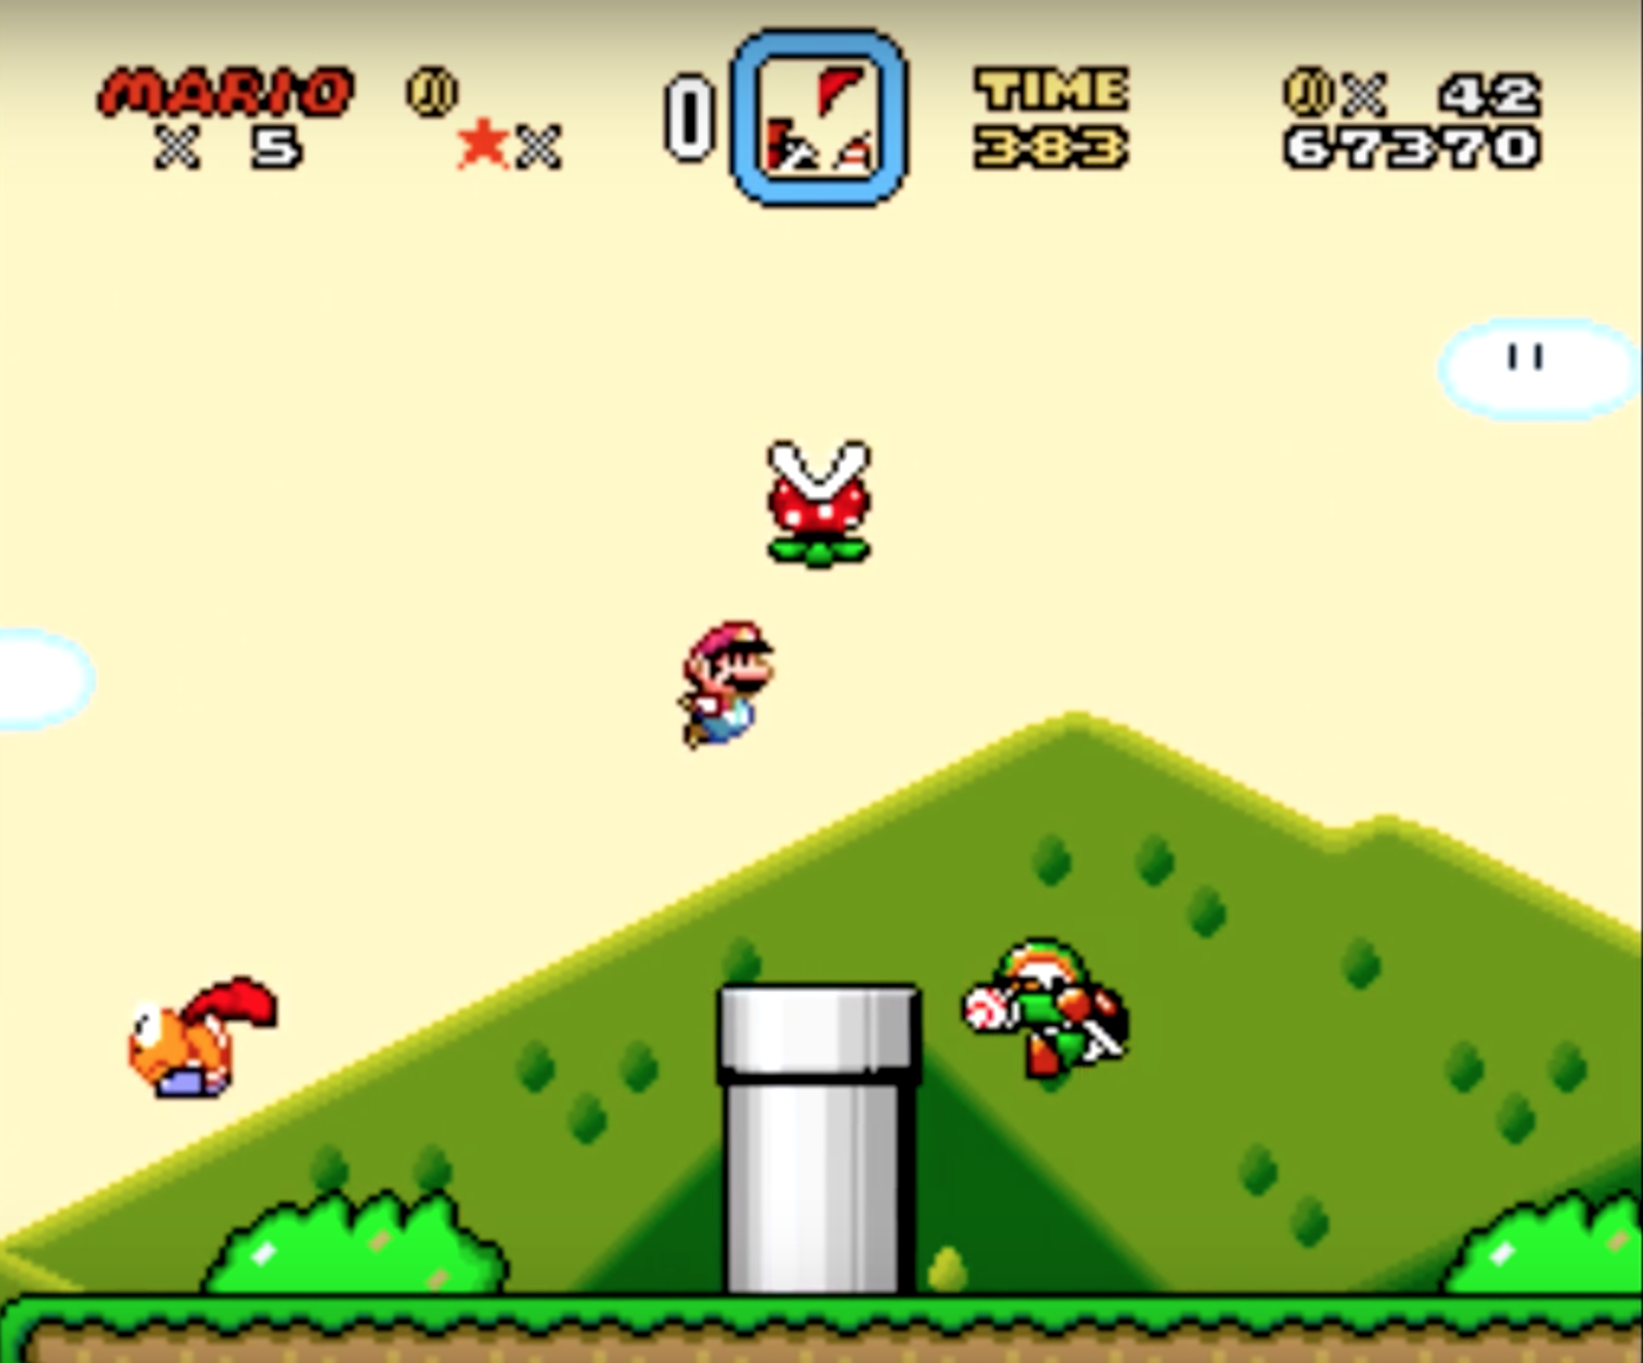
\includegraphics[width = \textwidth]{MarIO.png}
	\caption{MarI/O}
	\citep{MarIO} 
\end{figure}
%Probably need to ask for permission to use that 
%Sent a message on facebook to request permission

Despite that description, the intelligence of MarI/O is questionable. Although it has mastered the art of manoeuvring its way across the level in question, that is all it has done. In other words, if we were to take the same agent and run it on another Super Mario level, it wouldn't do so well. It has figured out how to pass through the level by continually moving right, and jumping at optimal times to avoid enemies and gaps in the map. Albeit successful, this is not a strategy that could be deemed as \textit{intelligent}.\\

For Alan Turing to consider a machine intelligent, it must be able to act in a way that would be indistinguishable from the way a human would act. The Turing Test, created by Turing himself in 1950, was an imitation game whereby a human would hold textual conversations with another human, and with a computer. If the testing human is unable to successfully differentiate between the two based on interrogation within those conversations, then Turing would deem it unreasonable not to call the computer intelligent\citep{TuringTest}.\\

Although dealing in a different realm altogether, applying the same principle to MarI/O and questioning if the strategy it presents could pass a similar test of human judgement to decide whether or not it is a strategy that is likely to have been played by a human, then we cannot possibly declare MarI/O's technique as an intelligent solution.\\

Related videos include a Unity3D project that uses NeuroEvolution of Augmenting Technologies (NEAT) to teach a car model how to drive around a purpose-build track\citep{26}, and another neural network that plays Mario Kart 64\citep{27}. Furthermore, there is an interesting tutorial series entitled, \enquote{Python Plays: Grand Theft Auto V}\citep{28}, which makes use of TensorFlow\citep{17}.\\

%Particularly card games
\subsection{Why Neural Networks?}
This project has dealt a hand presenting a problem in which a decision making process will have to make use of imperfect information. Not only can neural networks cope with this, in fact, they excel in situations of imperfect information.

Without a neural network, any given scenario within a problem would need to have some kind of hard-coded solution that is step-by-step in nature. Through a learning process, a neural network can find solutions to these scenarios on its own, via exploration of the possibilities thrown up by its decision making process over several generations. 

Imagine having to write the code for a solution to every single possible game state in Chess. For every move, you would have to write a solution for it as many times as there are possible opportunities for that particular move, i.e, every possible board configuration in which that single move is legal. This would take an unthinkable amount of time, and in reality is probably not even possible. Providing a coded solution for every possible board configuration would require a huge amount of code segments declaring that if some state condition is true, then do move this piece to this location. In doing so, we would find ourselves with an enormous file size, requiring unrealistic amounts of memory to run the code. 

On top of that, it could take the machine a long time to search through all of the conditions to find the one that applies to the situation at hand. 

In Chess, there are 400 configurations possible after each player has made a single move each, and over 72,000 after two each\citep{20}. This continues to grow at an exponential rate, making it easy to see why implementing a fully coded strategy is unrealistic. Additionally, this renders using a search tree for exploration of the full search space infeasible\citep{29}. Using a neural network and allowing it to analyse every situation it encounters on its own, deciding what moves to make and learning from the results is a far better idea. 

Additionally, hard-coding solutions to given situations would make the game predictable, and could also lead to making moves that are not actually the best for that current game state. The flexible nature of a neural network provides the potential to reach better solutions that hard-coding might miss out on. 

In our Switch card game for example, there is a rule that states if the previous player played a 2, you must pick up two cards unless you have another 2. Knowing this, and wanting to force our opponent to inherit more cards, we might hard-code a strategy that says, \enquote{if you have a 2 and it is available to be played, play it.} This could cost us a chance to win the game though! 

If we only had two cards left, both of the same suit and matching the suit of the most recently played card, one being a 2 and the other being a 7, we could play the 7 first, and that would allow us to play a run of that suit. This would allow us to play both cards and win the game. A neural network might learn that playing a 7 is better than deploying a 2, but our hard-coded strategy may not.\\

%*****what have people used neural networks for with control problems and how is it related to my problem******\\

Alter\citep{21} is another example implementation of artificial neural networks. Replicating the upper-body of a human, Alter is a robot that can almost be described as being \textit{alive}. 

Technologically, it consists of 42 pneumatic actuators and a \enquote{central pattern generator} with a neural network used to let the robot develop movement patterns\citep{21}. The network receives input in the form of sensory data relating to temperature and humidity as well as proximity and noise\citep{22}. 

Although it does not behave in a human-esque manner, Alter is continually perceiving the nearby environment, and reacting to it in such a way that is completely uncontrolled by a human, and not pre-programmed. This is how it somewhat provides the illusion of life. \\

RoboCup\citep{23} is a robotics competition whereby robots compete in a game of football (soccer). The competition was launched by Japanese researchers in 1993, who soon after found themselves inundated with requests from other nations to make the project an international joint effort\citep{23}. 

RoboCup Soccer is an annual competition, and the performance of contestants is seen to increase across the various leagues yearly\citep{30}. Each league has a different type of robot, and so certain league alternate artificial intelligence problems with respect to the way in which they interpret and play the game. For example, not all of the leagues have robots with human-style bodies, and instead have wheels and 360$\degree$ vision. These variations allow for the RoboCup competition to encourage and facilitate research into an array of varying aspects within the artificial intelligence field. 

As the robots that participate in these competitions vary in size and shape, detecting fellow robots visually is not a simple task. It is however a job for a neural network of multi-layer perceptrons\citep{24}. Robots should also be able to recognise team-mates and tell them apart from opposing players. 

In terms of playing the game, it is infeasible due to the dynamic nature of the game to consider all situations ahead of time when programming the robot\citep{25}. Machine learning is therefore a necessity for RoboCup participation.\\

To demonstrate the significance of neural networks in the real world, let's look at an open source software library that is used worldwide. 

Google initially developed TensorFlow, the successor to the DistBelief system they used from 2011\citep{19}, for research in neural networks and machine learning\citep{17}, but has since grown into a much wider-serving interface. It has found itself deployed in complex computational areas such as speech recognition and natural language processing, as well as image recognition\citep{18}. 

Google themselves use TensorFlow for a variety of different projects;  Massively Multitask Networks for Drug Discovery and RankBrain are examples of large-scale deep neural network projects owned by Google, used for drug discovery and information retrieval respectively\citep{17}. 

Other companies which benefit from the use of TensorFlow include Nvidia, Snapchat, Intel, Twitter, Dropbox, Ebay and Uber to name a few. \\

%RELATE IT TO A (CARD) GAME 

\subsection{Why Evolve Neural Networks?}
Artificial neural network evolution has demonstrated positive results with tasks involving reinforcement learning, and has performed especially well with those that include hidden state information\citep{EfficientEvolutionOfNeuralNetworkTopologies}. This appeals to the needs of this project as it deals with unknown game aspects, such as the cards in other people's hands. 

The evolution of neural networks has demonstrated a large degree of potential when coupled with tasks solvable by reinforcement learning techniques\citep{EfficientEvolutionOfNeuralNetworkTopologies}. It outperforms the basic methods of reinforcement learning against tasks that are considered benchmarks, and is therefore a justifiably sought after means of decision making.\\

Another arcade-style game that has been used in the research of neural networks is PAC-MAN. In a particular paper introducing the concept of trying to evolve a player for the retro classic, a simple ghost avoidance strategy was given a hard-coded implementation for comparison purposes. Perhaps expectedly, the results were underwhelming - in particular when compared to other implementations in the same project. The aim was to demonstrate that the neural networks were learning something more sophisticated than such a simple strategy\citep{MSPacMan}. Evolving neural networks and allowing the controller to develop its own strategies, as opposed to hard-coding them, produced universally superior results.\\

Evolved neural networks are not without disadvantages. Their black-box nature means that we don't get an understanding of why it makes certain decisions or takes particular actions, and it can be difficult to modify behaviours. Furthermore, there is the problem of potential overfitting, as previously described with the MarI/O\citep{MarIO} example where the agent has perfected that particular Mario map, but if it were to be placed in a new environment, the same strategy would not suffice. It would be the same as introducing a robot of never before seen size or shape in our RoboCup\citep{24} example, without allowing retraining with images of the new robot machine.\\

\subsection{Why Co-Evolve Topologies and Weights?}
Much like when we compare evolving neural networks to standard reinforcement learning techniques, evolving network topologies often performs in a significantly superior manner to the alternative - in this case fixed topology neural network evolution\citep{EfficientEvolutionOfNeuralNetworkTopologies}. 

There is always a chance with evolving topologies of making the search overly complex, but in contrast to that possibility there is also the potential to find the optimal amount of hidden nodes for any given problem by itself, which would save some time\citep{EfficientEvolutionOfNeuralNetworkTopologies}. It is also possible for NEAT to reduce the complexity of a network's structure when evolving the topology. 

Rather than searching through topology space using a brute force approach, NEAT begins with small, simple networks before expanding the search space only when necessary\citep{EvolvingARovingEyeForGo}. This strategy attempts to counter the problem of overfitting, and the flexibility is what allows it to find far more complex controllers than evolution networks with a non-negotiable topology.\\

%RELATE IT TO A (CARD) GAME \\

\subsection{Summary}
%Given previous work it suggests that NEAT will be an appropriate algorithm for solving this problem
%The unanswered questions (that we will go on to answer):
%-How intelligent is the solution
%-How many generations did it take
%-How computationally complex is it regarding hidden layers and topology. 
Evolving artificial neural networks, including structural network evolution, allows us to create solutions that perhaps would not be feasible to build with step-by-step hard-coding approaches. For a project such as this where we cannot write a fool-proof strategy to deal with any given situation within the game, it is ideal to have tools such as NEAT. 

Despite the disadvantages and complexities of evolved neural networks, the negatives are outweighed by positives. They are able to achieve things that developers alone cannot, and so it would be difficult and perhaps unwise to overlook them for some projects, particularly those with huge search spaces like Chess and Go.  

As Switch is largely down to luck like most (if not all) card games, there is never going to be a perfect solution. That said, the aim of this project is to see whether evolved neural networks are more capable of finding a consistently positive solution than a programmer implementing a strategy in advance could be. 

\newpage
\section{Methodology}
%And so on for each of the chapters.  The template automatically starts new chapters on a new page.  The associated guidelines tell you what the available styles do and also how to structure a report.
%There is a section break on this page that you should be careful NOT to delete otherwise the references and appendices will be numbered continuously with the rest of the document.

\subsection{Language and Libraries}
The programming language used to build this project is C++. It is used in collaboration with the NeuroEvolution of Augmenting Topologies (NEAT) library. 

\^ Following a tutorial that I can't seem to find the download link to the .ps file but I've uploaded the converted pdf to my website\\



The graphical aspect was developed using an import of the Simple and Fast Multimedia Library (SFML), with playing card textures courtesy of Kenney Vleugels, found here:\\ https://opengameart.org/content/boardgame-pack
\begin{figure}[h]
	\centering
	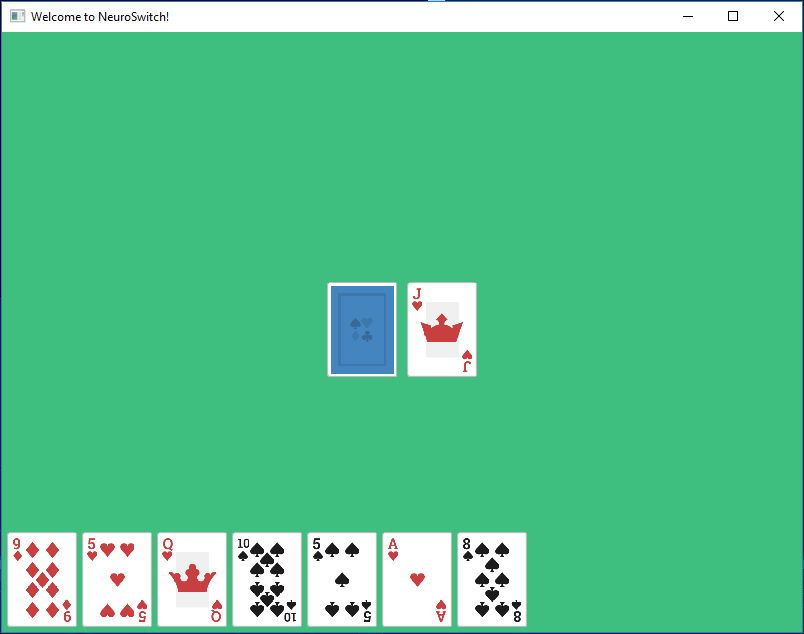
\includegraphics[width = \textwidth]{SFML.png}
	\caption{Game UI}
\end{figure}


\subsection{Design}
Design patterns / class diagrams and such for my code

\begin{figure}[h]
	\centering
	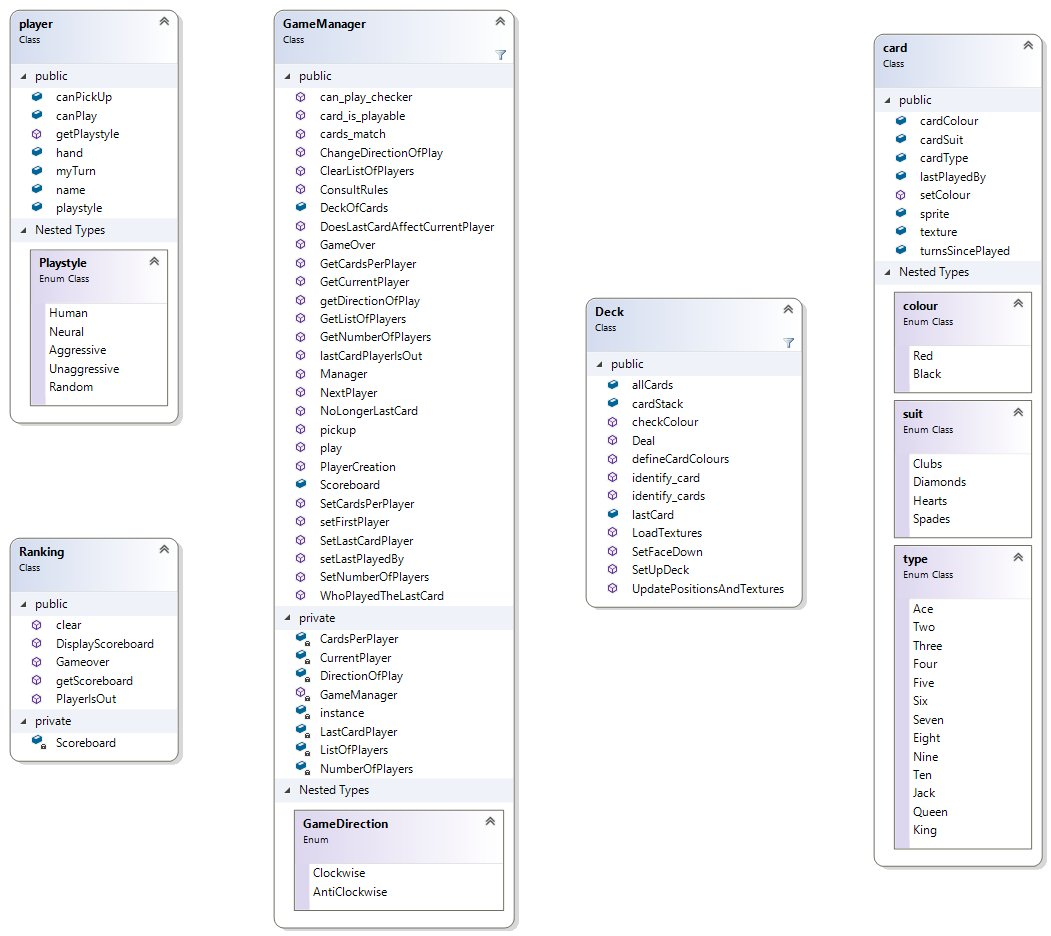
\includegraphics[width = \textwidth]{ClassDiagram.jpg}
	\caption{Game Class Diagram}
\end{figure}

Figure 12 helps to visualise the code structure behind the game, showing the five classes and their member functions. 

The Game Manager singleton class is central, with its deck of cards object class on the right. For the sake space and readability, 105 card and texture objects have been omitted from the image. The specifics of what a card object is made up of can be seen on the far right.

Looking back on the other side of our singleton, we see the ranking system and a look at the components of a player object. \\

I can't help but feel that these should have relationship lines, but I couldn't figure out how to add them. D: \\


As seen in the diagram, the game management class is the hub that interacts with everything throughout each match. It is an integral part of the game operation, and needed to be accessible by most of the classes. This meant that circular dependency issues were going to arise, and so the need for a singleton class was established. 

With all necessary classes being able to access the same instance of the game manager class whenever it was necessary made things a whole lot easier than trying to find a way around circular dependency problems. 
\subsection{Neural Network}
Could've started from scratch rather than use NEAT, but used it for reasons X Y Z

NEAT has special crossover operations cause taking half of a NN and sticking to another one probably won't perform well 

\subsection{Evolutionary Algorithm}

\subsection{Fitness Evaluation}


\newpage
\section{Results}
%Hardcoded stuff\\\\
When the underlying game foundation had been built, it only allowed for human vs human interaction. This meant testing was not only very click-intensive, but also extremely time consuming. As a result, some automatic playability was implemented to allow for speedy, hands-free testing. The automatic players were given hard-coded strategies for playing the game, aptly named, 'Aggressive,' 'Unaggressive,' and 'Random.' 

The aggressive player will check their hand for cards that will inflict the most damage to their opponents, before just selecting the first legal card in the hand if none are available. Unaggressive does the opposite. It actively avoids playing twos, eights and black queens unless no other playable cards are contained in their hand. Random players will just shuffle their hand before choosing a playable card.\\

Once the game had been thoroughly tested and all bugs eradicated, work on the final player type was to ready to be begin. Of course, the 'Neural' player was going to be playing against the hard-coded play-styles, as well as potentially facing humans in future. For this reason, a baseline of hard-coded performances was measured. The strategies were tested against one another in a one on one format, before a free for all between the three.\\

Below are a series of tables depicting the results of this testing.\\

\begin{table}[h!]
	\begin{tabu} to \textwidth { | X[c] | X[c] | X[c] | }
		\hline
		Games Played & Aggressive Wins & Unaggressive Wins \\
		\hline
		1000  & 552	& 448 \\
		\hline
	\end{tabu}
\caption{Hard-coded Results | Aggressive vs Unaggressive}
\label{table:1}
\end{table}

\begin{table}[h!]
	\begin{tabu} to \textwidth { | X[c] | X[c] | X[c] | }
		\hline
		Games Played & Aggressive Wins & Random Wins \\
		\hline
		1000  & 501 & 499 \\
		\hline
	\end{tabu}
\caption{Hard-coded Results | Aggressive vs Random}
\label{table:2}
\end{table}

\begin{table}[h!]
	\begin{tabu} to \textwidth { | X[c] | X[c] | X[c] | }
		\hline
		Games Played & Random Wins & Unaggressive Wins \\
		\hline
		1000  & 539 & 461 \\
		\hline
	\end{tabu}
\caption{Hard-coded Results | Random vs Unaggressive}
\label{table:3}
\end{table}

As expected, the more attacking player had the most success. However, I was taken aback to discover it only won 55.2\% of 1000 games against the unaggressive player affectionately known as 'Passive Pete.' This was less surprising, though, than the difference between 'Angry Adalia' and 'Random Rachel!' I had predicted a landslide victory for aggressive, but had the random strategy won just a single game more, it would've been a tie over 1000 iterations. I think these results in particular are testament to the unpredictability of Switch. 

The remaining battle was between Random Rachel and Passive Pete. There is not a lot to be said about this. An unaggressive approach to the game is effectively allowing the opposition to play without being severely punished, and deserves to yield poor results. Similarly, the random approach is totally unpredictable, and so this contest could probably go either way if repeatedly tested.\\

Finally, the ultimate showdown; Aggressive vs Unaggressive vs Random. 

\begin{table}[h!]
	\begin{tabu} to \textwidth { | X[c] | X[c] | X[c] | X[c] |}
		\hline
		Games Played & Aggressive Wins & Unaggressive Wins & Random Wins\\
		\hline
		1000  & 346	& 314 & 340 \\
		\hline
	\end{tabu}
	\caption{Hardcoded Results | Aggressive vs Unaggressive vs Random}
	\label{table:4}
\end{table}

As the results show, the aggressive play-style is the most successful. However, the margin of victory was somewhat surprising.\\

\subsection{Agent vs Hard-coded Strategy}
-Population of 20-50 initially - could be something we grow experimentally

-100-150 generations

-30 replicates of these generations 

\subsubsection{Neural vs Unaggressive}
.
\subsubsection{Neural vs Random}
.
\subsubsection{Neural vs Aggressive}
.

\subsection{Agent vs Human(s)}
[Future work] move to evaluation 

\subsection{Agent vs Agent}
[Potential future work]

\newpage
\section{Critical Evaluation}
\begin{itemize}
	\item Gantt chart from beginning of project
	\item Gantt chart from week 9 milestone (ie now, when lit review is done)
	\item Gantt chart at Christmas/New Year
	\item Completed project gantt chart 
\end{itemize}


\begin{figure}[h]
	\centering
	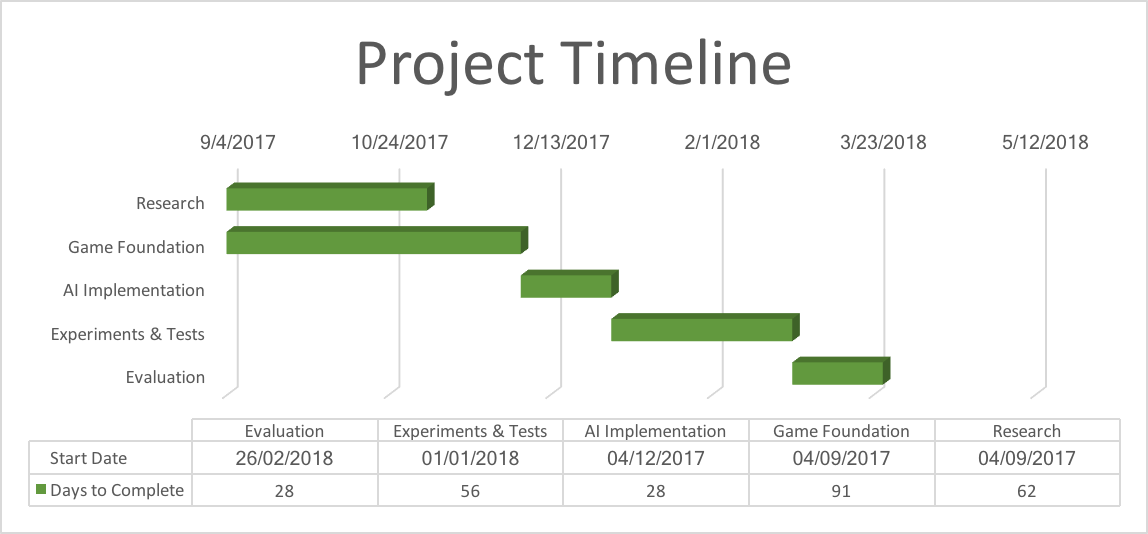
\includegraphics[width = \textwidth]{Gantt1.png}
	\caption{Original Project Timeline Gantt Chart}
\end{figure}

\begin{figure}[h]
	\centering
	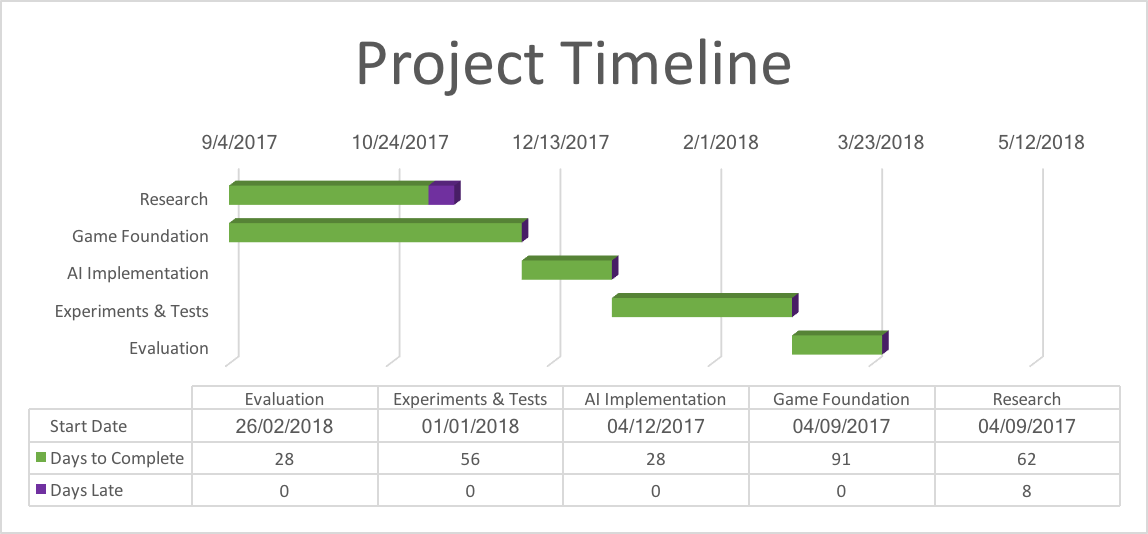
\includegraphics[width = \textwidth]{Gantt2.png}
	\caption{Updated Gantt Chart - New Year}
\end{figure}

The research phase of the project ran a little over the initial prediction, but as it ran concurrently with game development, I was able to recover without any early knock-on effects. The foundation of my card game had always been targeted for completion by Christmas - and the final bug was crushed in the small hours of the morning on boxing day. 

\begin{figure}[h]
	\centering
	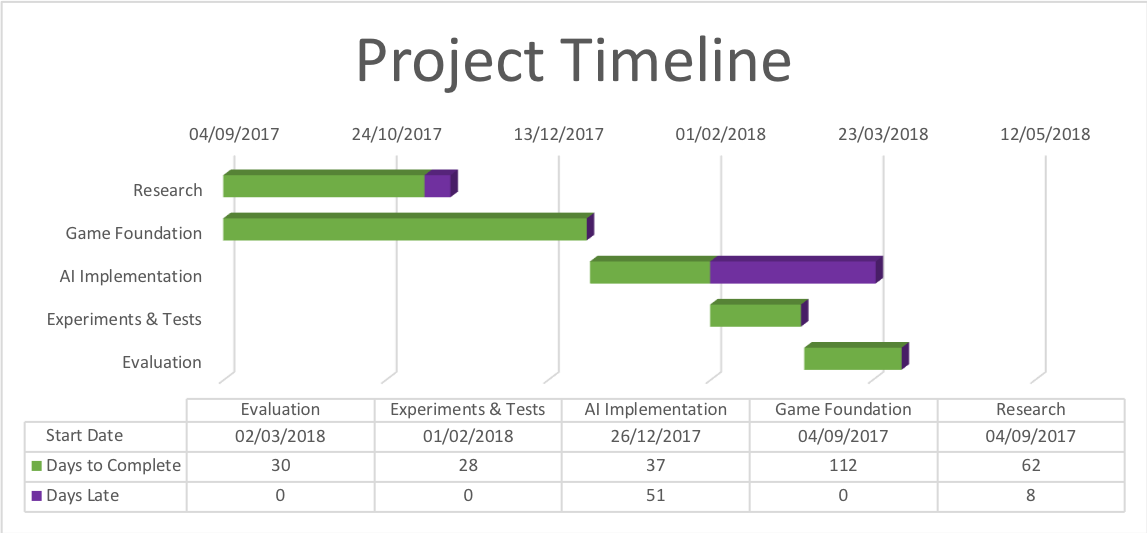
\includegraphics[width = \textwidth]{Gantt3.png}
	\caption{Post-AI Project Gantt Chart}
\end{figure}

AI implementation took far longer than anticipated, and so the final two stages had to be re-evaluated for the final stretch. 

\begin{figure}[h]
	\centering
	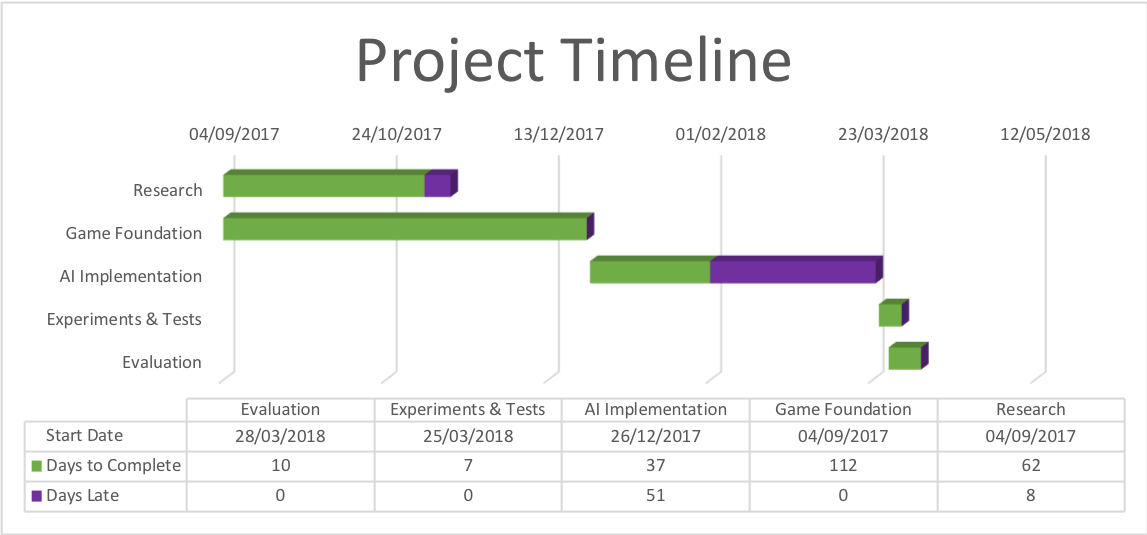
\includegraphics[width = \textwidth]{Gantt4.png}
	\caption{Complete Project Gantt Chart}
\end{figure}



\newpage
\section{Conclusion}


\newpage
\bibliographystyle{plainnat}
\bibliography{Citations}
%example of References. See https://en.wikibooks.org/wiki/LaTeX/Bibliography_Management
%might be good to use a separate document for these so your main work is not one really long text file. 

%you can crate this on a extra tex document just like the title or any other part of the document.

\newpage
\renewcommand{\thepage}{}
\begin{appendices}
\section{Project Overview}
%insert IPO 

\Large{\textbf{Initial Project Overview}\\

\textbf{SOC10101 Honours Project (40 Credits)}}\\                                                      

\large{\textbf{Title of Project:}}

\normalsize{Evolution of Neural Network Controllers for Gameplay Behaviours} \\

\underline{\textbf{Overview of Project Content and Milestones}}

The idea is to implement a card game with four players. One of the players is the human, another is an AI agent that has no idea how to play the game, and the other two are hard-coded to know the rules and how to play. The intention is for said card game to be Switch, however this is subject to change if the rules are found to be too difficult for the scale of the project – in which case a simpler game will be substituted in.


The agent then learns how to play by trying to make moves based on neural networks. Initially this will be totally random but after the first generation of the algorithm cycle, it will be based on the chromosomes with the highest fitness, which should then begin to provide better results. These moves can be blocked if they are not legal. There'll be a scoring system for the agent that will be negatively affected by illegal moves and it will then use this to learn how to do better the next time it plays. The scoring system will also see the agent penalised for losing or not winning. This will be what our fitness is based on. 


It is worth noting that how successful you are in a game of Switch depends entirely on the hand you’re dealt, and how your opponents play the hands they are dealt. A lot of the game is about luck, and so negatively affecting the agent’s score should take this into account and deploy some leniency. 


The project will make use of the NeuroEvolution of Augmenting Topologies (NEAT) library and will most likely be coded in C++. It will use neural network controllers, co-evolving weights and topologies. \\

\pagebreak
\large{\textbf{The Main Deliverable(s):}}
\begin{itemize}
	\item A playable card game that incorporates an Artificial Intelligence agent that must learn how to play the game from scratch based on a score system that penalises the agent for illegal or costly decisions. 
	\item Experimental research into improving the performance (in terms of score) or speeding up the learning process of the agent. 
	\item A report into what positively or negatively affects the agent, and what causes the effects that it has including experiment results using charts and figures. Changes will be made by varying parameter settings of the evolutionary algorithm in a systematic way.
\end{itemize}

\large{\textbf{The Target Audience for the Deliverable(s):}}

Whilst the final product will be a playable game, it will really be aimed more at being experimental research into Artificial Intelligence techniques and, more specifically, evolving neural network controllers for playing games. Thus, the audience most likely to be interested in the project are those who also want to look into artificial intelligence agents. \\

\pagebreak
\large{\textbf{The Work to be Undertaken:}}
\begin{itemize}
	\item Design and build a game of Switch without the AI agent
	\item Thoroughly test the bare-bones game to ensure it works perfectly without bugs
	\item Research neural networks and evolutionary algorithms
	\item Implement the AI agent
	\item Experiment with a few different techniques and test how they perform in terms of improving or decreasing the agent’s intelligence/performance in game.
\end{itemize} 

\large{\textbf{Additional Information / Knowledge Required:}}

Neural networks and evolutionary algorithms\\

\large{\textbf{Information Sources that Provide a Context for the Project:}} %HATE how Project is on the next line here
\begin{itemize}
	\item Lubberts, \& Miikkulainen (2001). Co-Evolving a Go-Playing Neural Network.
	\item Stanley, Bryant, \& Miikkulainen (2005). Evolving Neural Network Agents in the NERO Video Game. IEEE Press.
	\item Thrun (1995). Learning to Play the Game of Chess. MIT Press. 
\end{itemize}

\large{\textbf{The Importance of the Project:}}

Exploring possibilities and limits of AI in games, particularly evolved controllers which do not have to be hard-coded.\\

\large{\textbf{The Key Challenge(s) to be Overcome:}}
\begin{itemize}
	\item Complete lack of knowledge and experience with Artificial Intelligence techniques
\end{itemize}

\newpage
\section{Second Formal Review Output}
%Insert a copy of the project review form you were given at the end of the review by the second marker

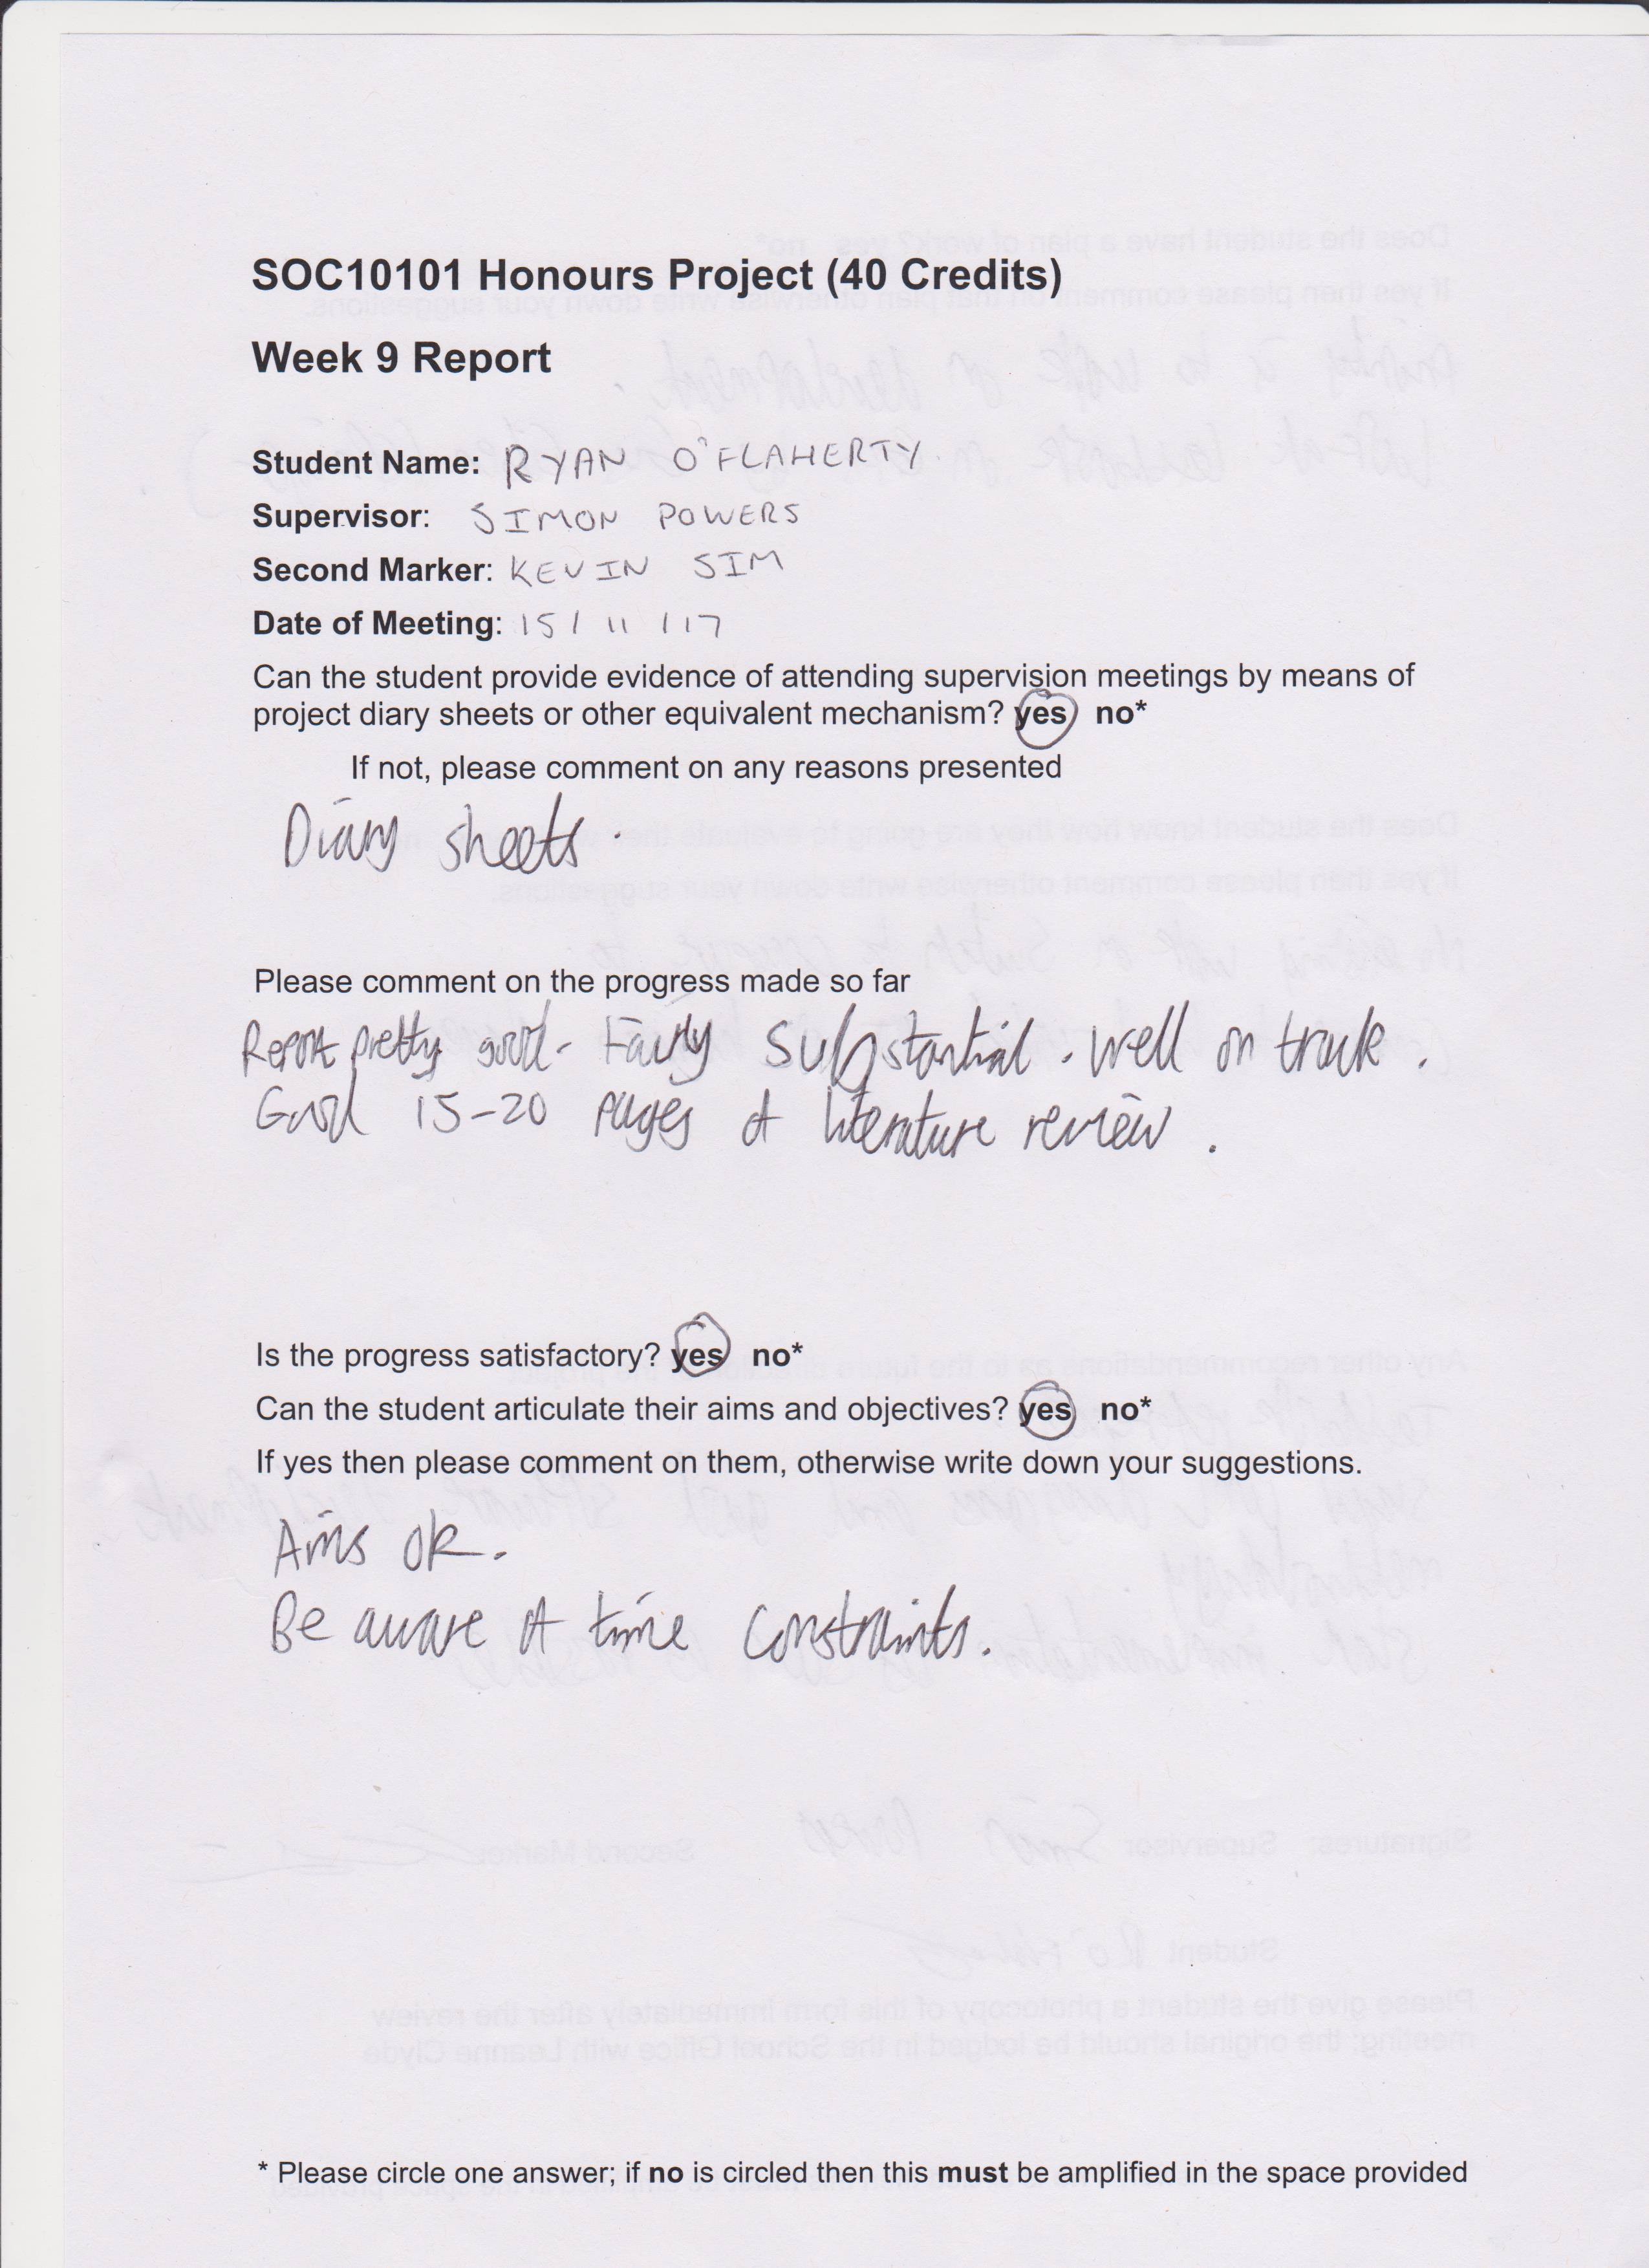
\includegraphics[width=\textwidth]{Week9Report1.jpg}

\newpage
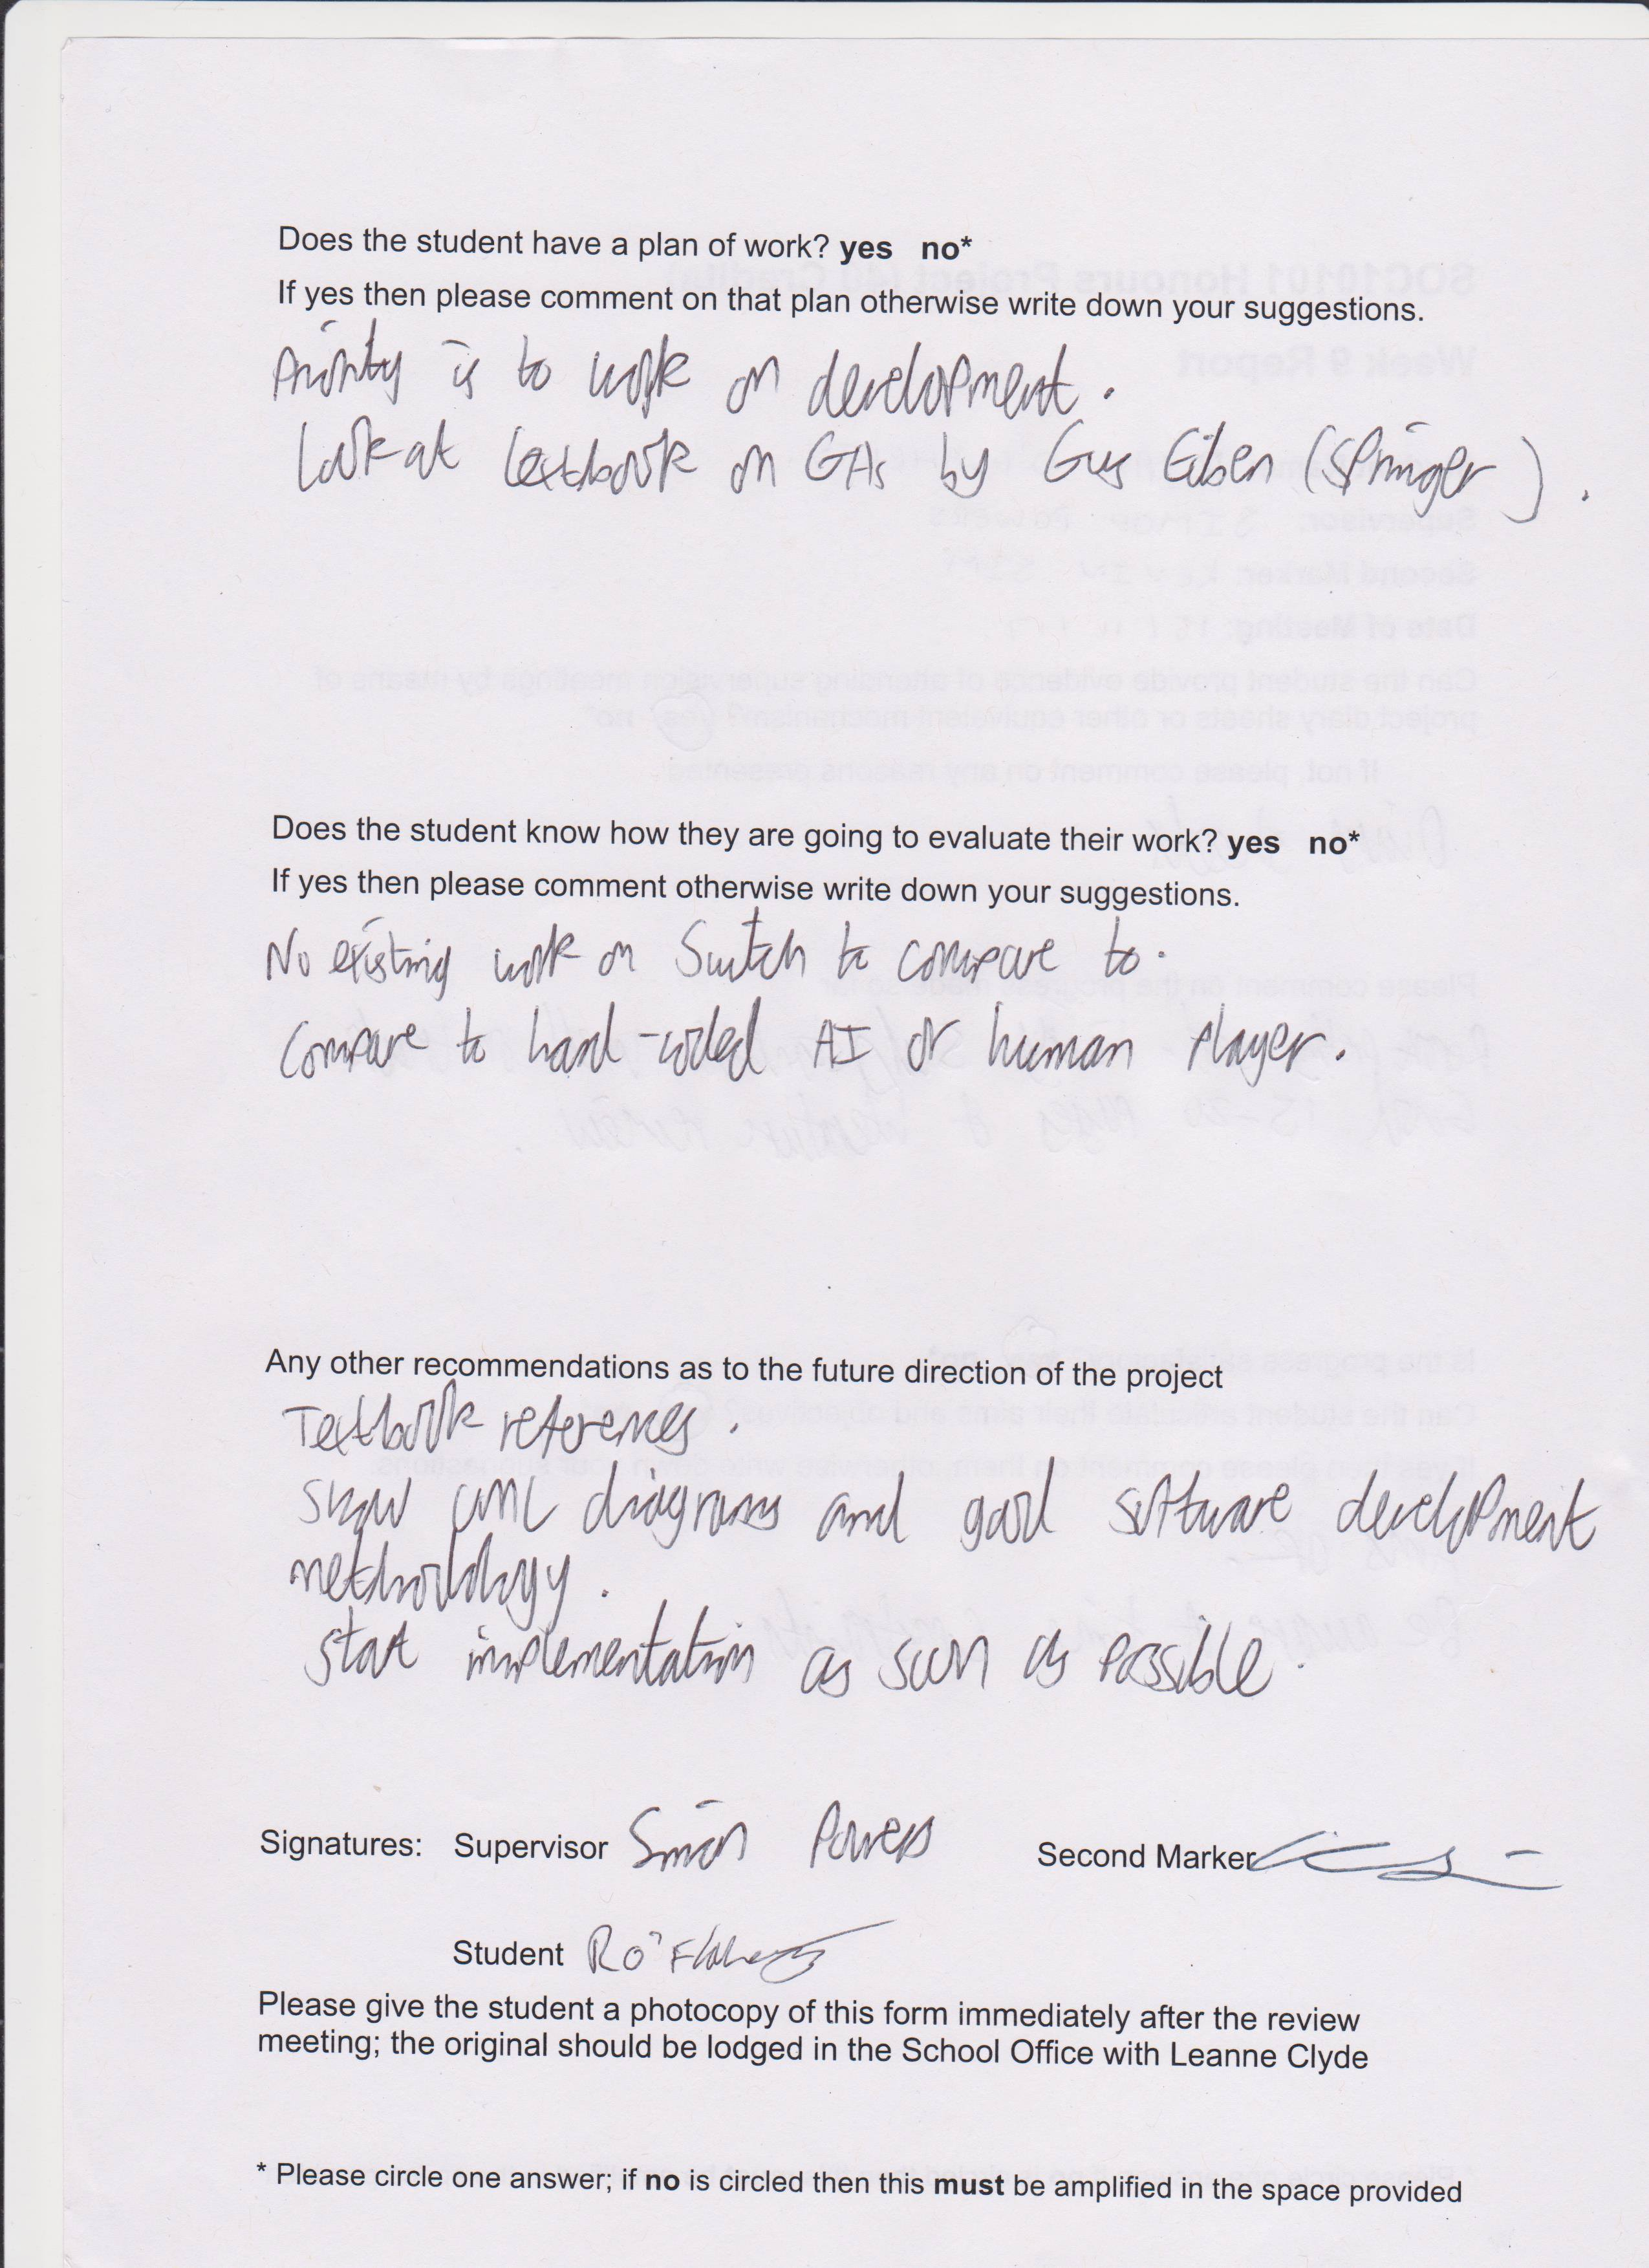
\includegraphics[width=\textwidth, height=\textheight]{Week9Report2.jpg}

\newpage
\section{Diary Sheets}
%(or other project management evidence)
%Insert diary sheets here together with any project management plan you have

%Includepdf starts on a new page which is kinda a pain
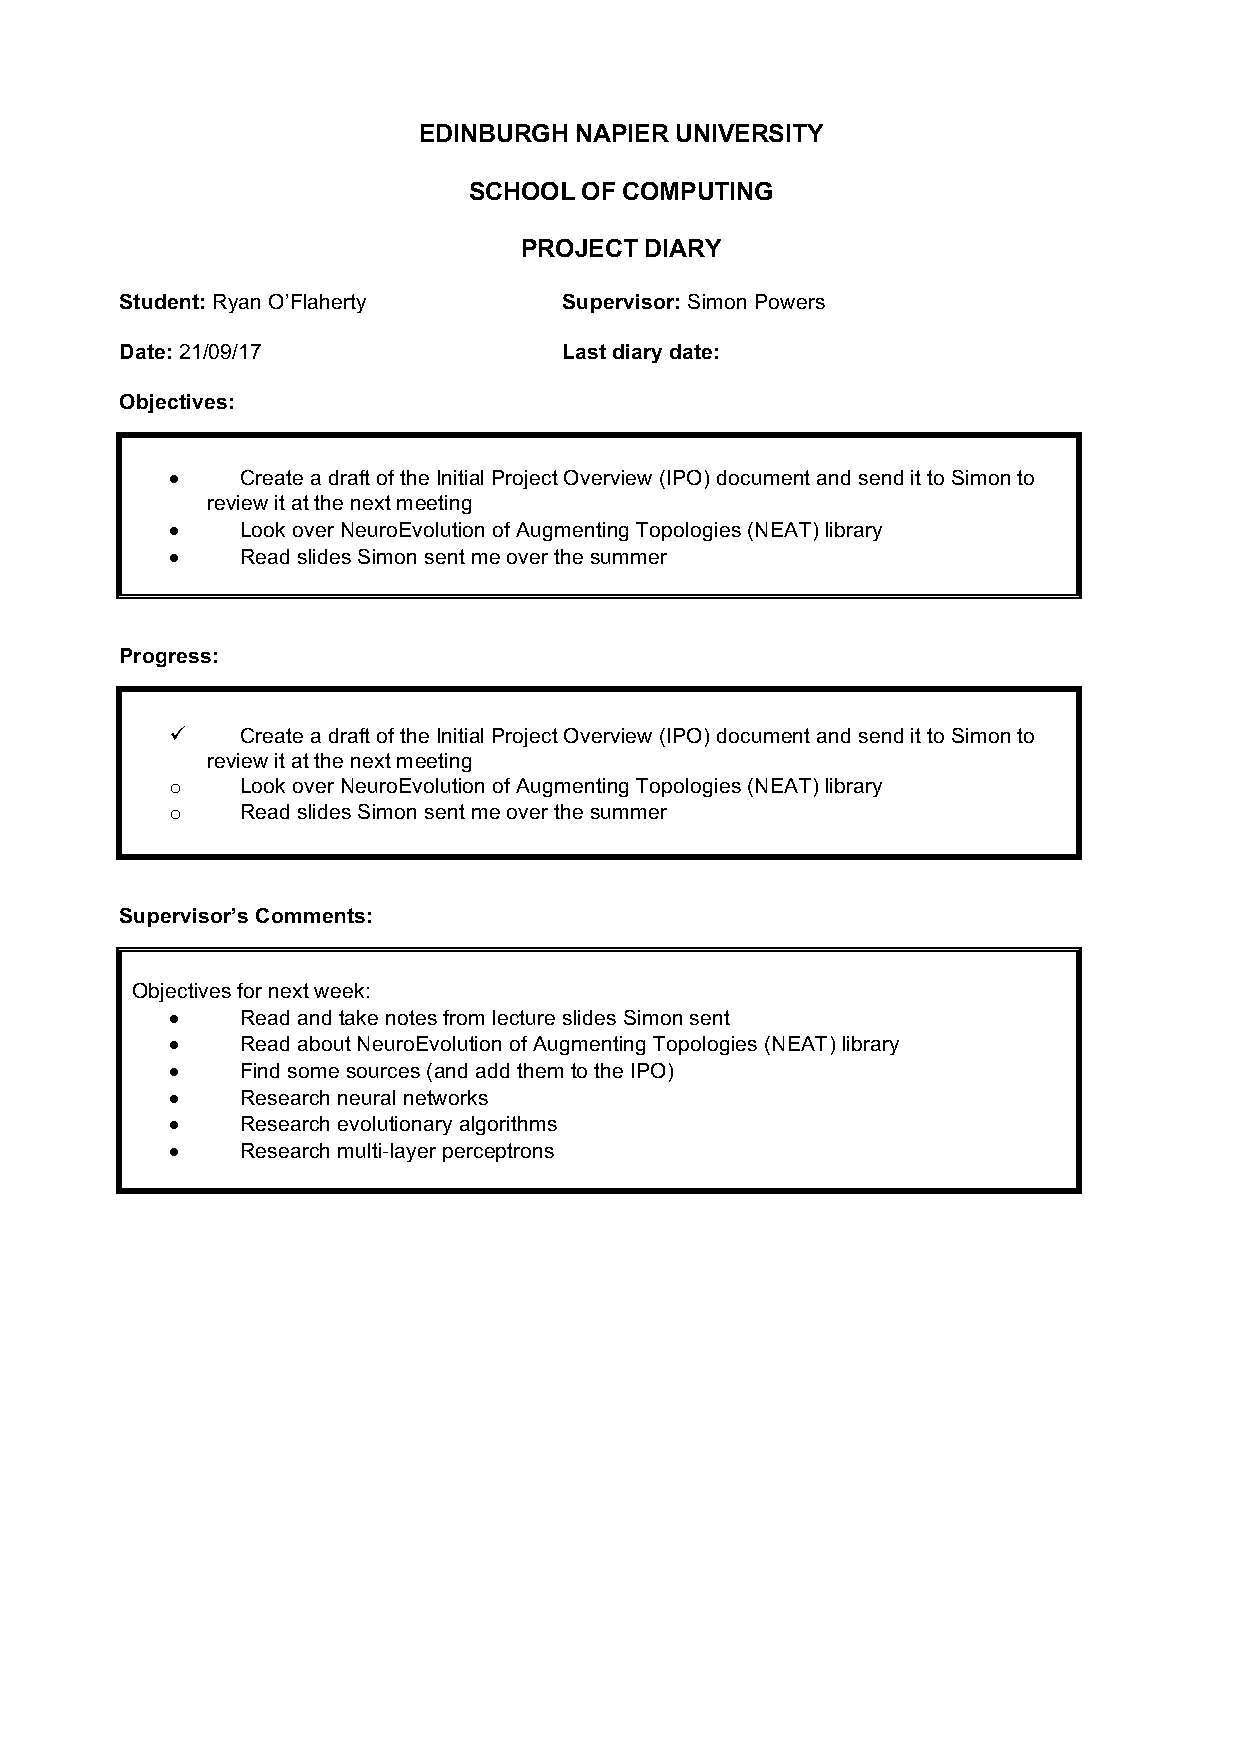
\includepdf[ pages=-,pagecommand={},width=\textwidth]{SupervisorMeetings/All.pdf}

\newpage
\section{Appendix 4 and following}
insert content here and for each of the other appendices, the title may be just on a page by itself, the pages of the appendices are not numbered, unless an included document such as a user manual or design document is itself pager numbered.
\end{appendices}

\end{document}
